\section{Experiments}
We first investigate the effect of different dynamics settings have on the performance. We then evaluate a few different matching algorithms to study the trade-off between stability, social welfare and consistency.
\subsection{Experimental Set-up}
% 0.5-1 page
% \begin{itemize}
%     \item Algorithms we are evaluating
%     \begin{itemize}
%         \item MPDA, WPDA
%         \item Probabilistic-based that always selects the best stable matching with a probability
%         \item Probabilistic-based that always selects the best matching with a probability
%         \item [Stretch] Deterministic algorithm that always selects the best sw with a consistency above a certain threshold
%     \end{itemize}
%     \item Dynamics
%     \item Number of agents, time steps, etc.
%     \item Evaluation set-up
% \end{itemize}
\paragraph{Dynamics Setting} For each agent, we independently initialize each utility value by sampling from a normal distribution $\mathcal{N}(\mu_u, \sigma_u^2)$ with scalar mean $\mu_u \in \mathbb{R}$ and variance $\sigma_u^2 \in \mathbb{R}$. For each utility value $x$, we clip it at 0 with $x \leftarrow \max(x, 0)$ to ensure it is non-negative. We further normalize the utilities such that each agent's utility vector has a total sum of 1. In addition, we independently sample each agent's excitement from a normal distribution $\mathcal{N}(\mu_e, \sigma_e^2)$. We clip the excitements at 0 such that the values are non-negative.

\paragraph{Algorithms} We implement both MPDA and WPDA~\cite{galeshapley1962}, which are guaranteed to return a stable matching. In addition, we implement a family of deterministic algorithms (Det) and a family of probabilistic algorithms (Prob, Prob-Stable), described as follows.

\textit{\textbf{Det}}: This is a family of algorithms parameterized by $c \in [0, 1]$ and returns a perfect matching with $$M^{t+1} = \argmax_{\mbox{consistency}(M^t, M) \ge c}{\mbox{sw}(M)}.$$
% In other words, the generated matching $M^{t+1}$ is the matching maximizing the social welfare subjected to the condition that the consistency is at least $c$ compared to the most recent match.
Solving for $M^{t+1}$ requires enumerating through all possible matching with consistency at least $c$. For computational efficiency, we perform the following approximation: we first identify and fix $N * c$ couples in $M^t$ that have the highest social welfare according to the updated utilities $\overrightarrow{u}^{t+1}$ and $\overrightarrow{v}^{t+1}$, and re-match the rest with the Hungarian Algorithm~\cite{Kuhn55thehungarian,Kuhn56thehungarian,Munkres1957Assignment} over the remaining men and women to obtain the maximum weight perfect bipartite matching, where the weight between a man node $m_i$ and a woman node $w_j$ in the bipartite graph is $u_i^{t+1}(w_j) + v_j^{t+1}(m_i)$. The generated new matching, which keeps at least the same $N*c$ couples from before, thus has consistency of at least $c$ and reasonably large social welfare.

\textit{\textbf{Prob}}: This family of algorithms is parameterized by a probability value $p$ and finds a matching as follows:
$$M^{t+1} = \begin{cases} \argmax_M{\mbox{sw}(M)} &\text{with probability $1-p$}\\ M^t &\text{with probability $p$}\end{cases}.$$
As a result, the expected consistency is at least $p$. We find $\argmax_M{\mbox{sw}(M)}$ by running the Hungarian algorithm on the full bipartite graph.

\textit{\textbf{Prob-Stable}} A variant of the probabilistic algorithm is to always return a \textit{stable} matching that has the maximum possible social welfare with probability $1-p$. However, in the case where we keep the previous matching $M^t$, since $M^t$ might not be stable with the updated utilities, Prob-Stable is not guaranteed to have stable matches all the time. One side note that it is infeasible to have the \textit{Det-Stable} variant, as stable matching might not exist for high consistency thresholds.


\subsection{Results and Analysis}
\begin{figure}
    \centering
    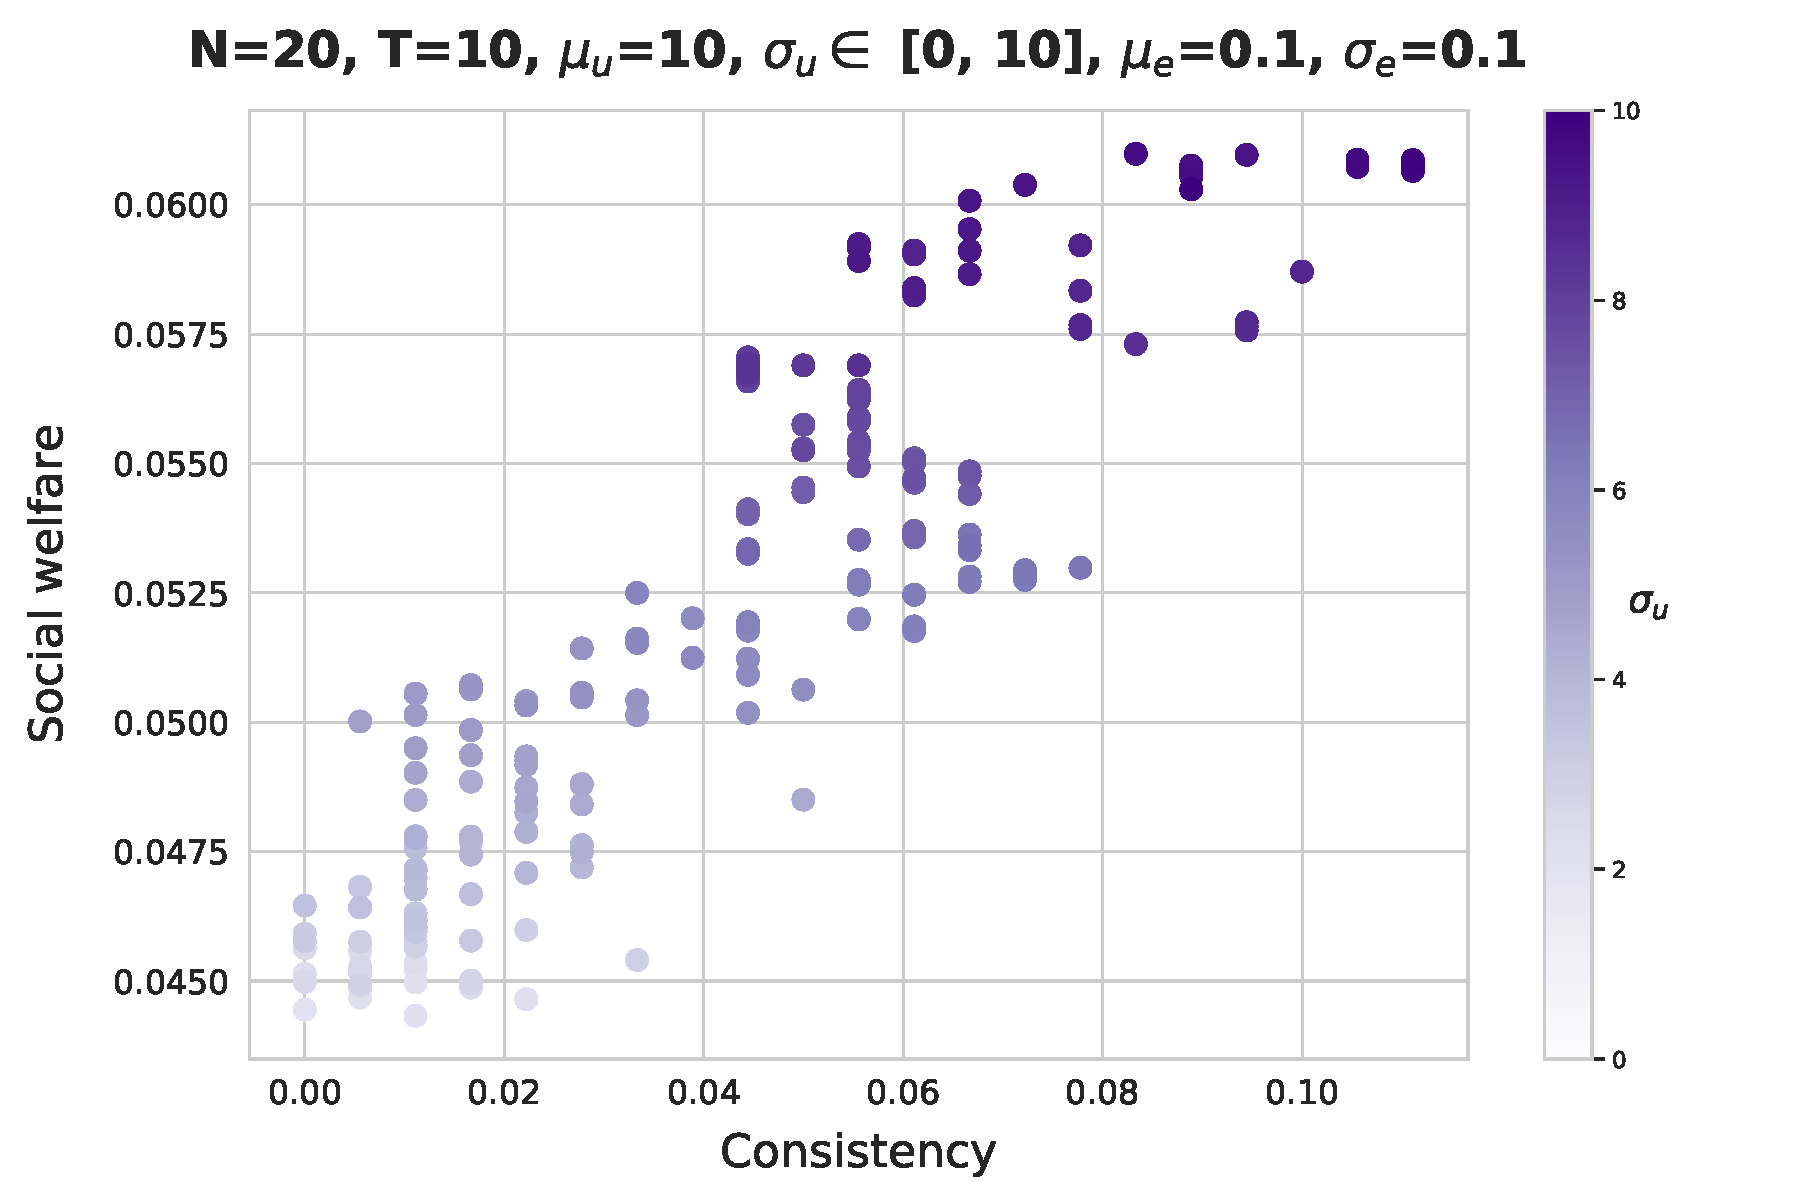
\includegraphics[width=0.32\linewidth]{figures/mpda_dynamics_initliazation.pdf}
    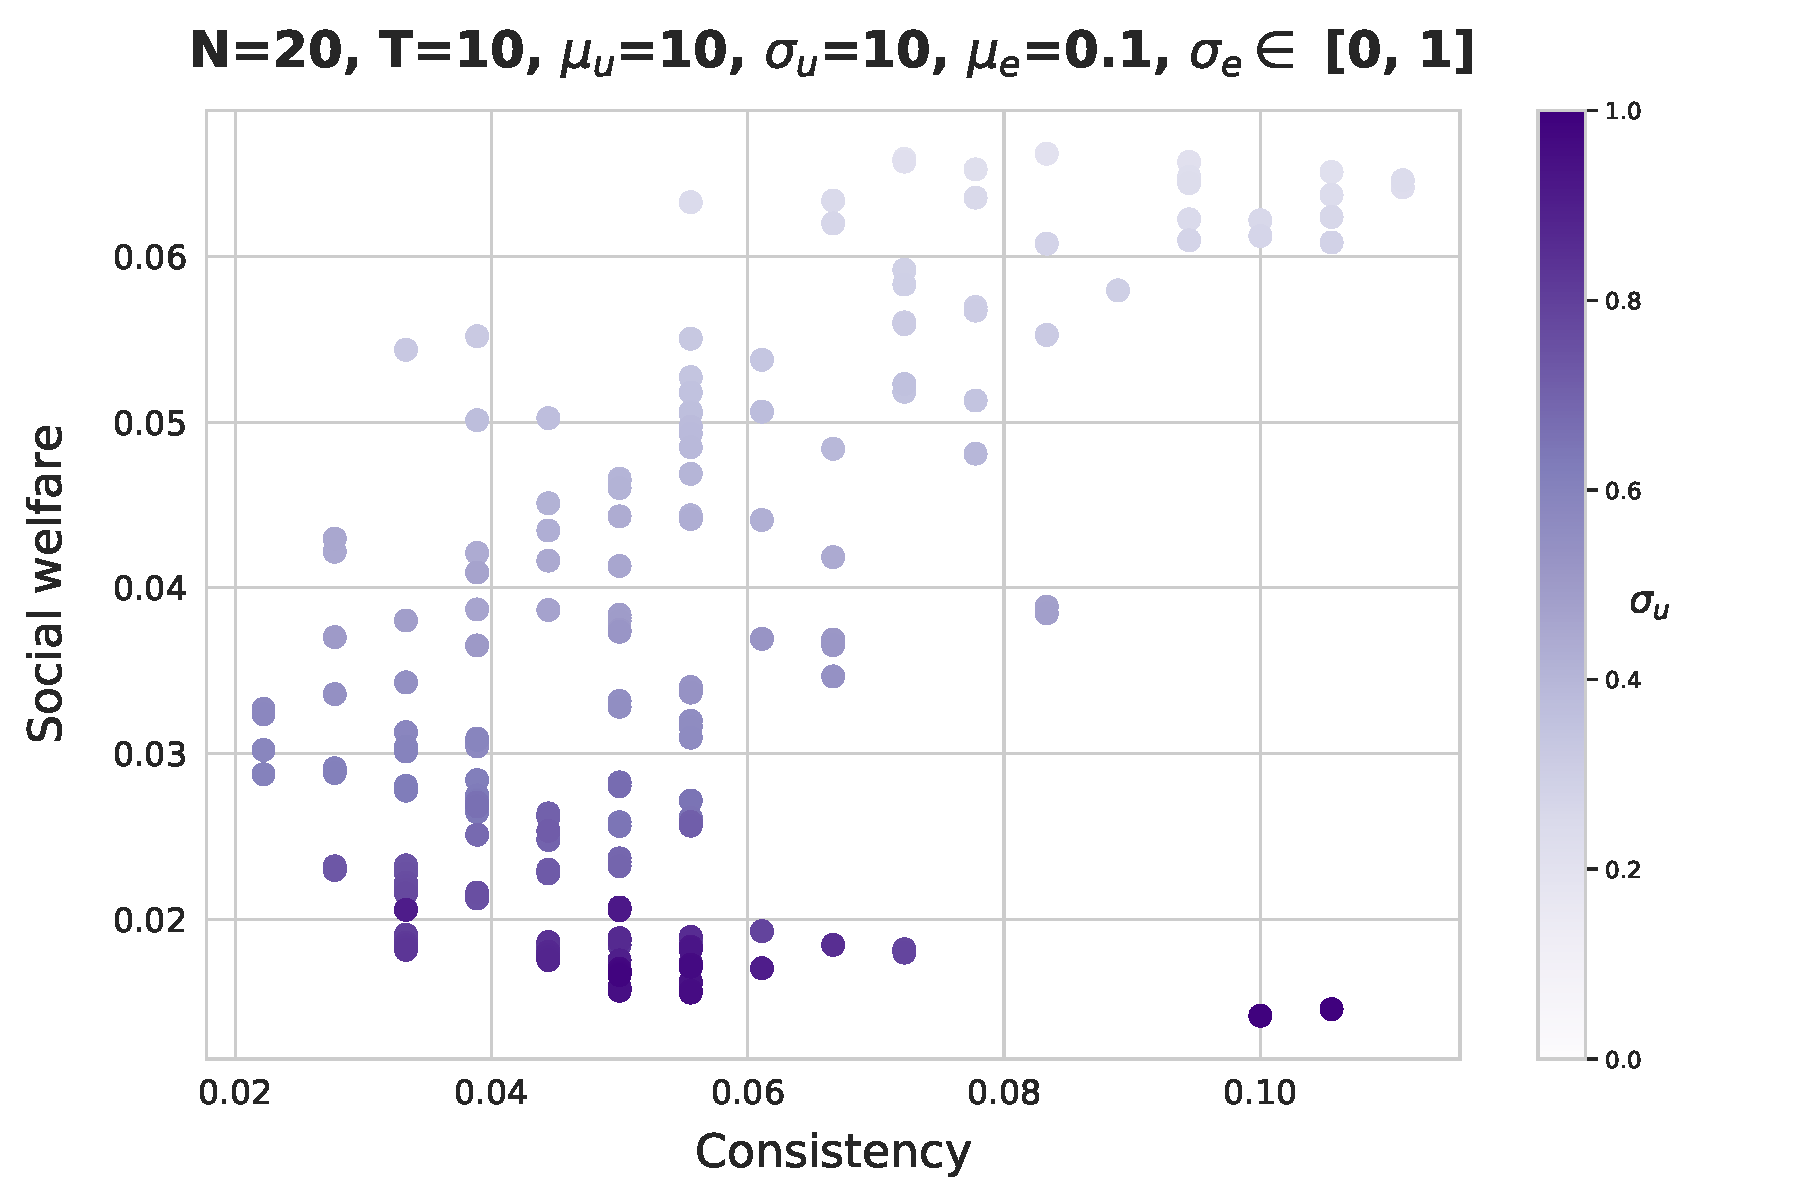
\includegraphics[width=0.32\linewidth]{figures/mpda_dynamics_excitement_std.pdf}
    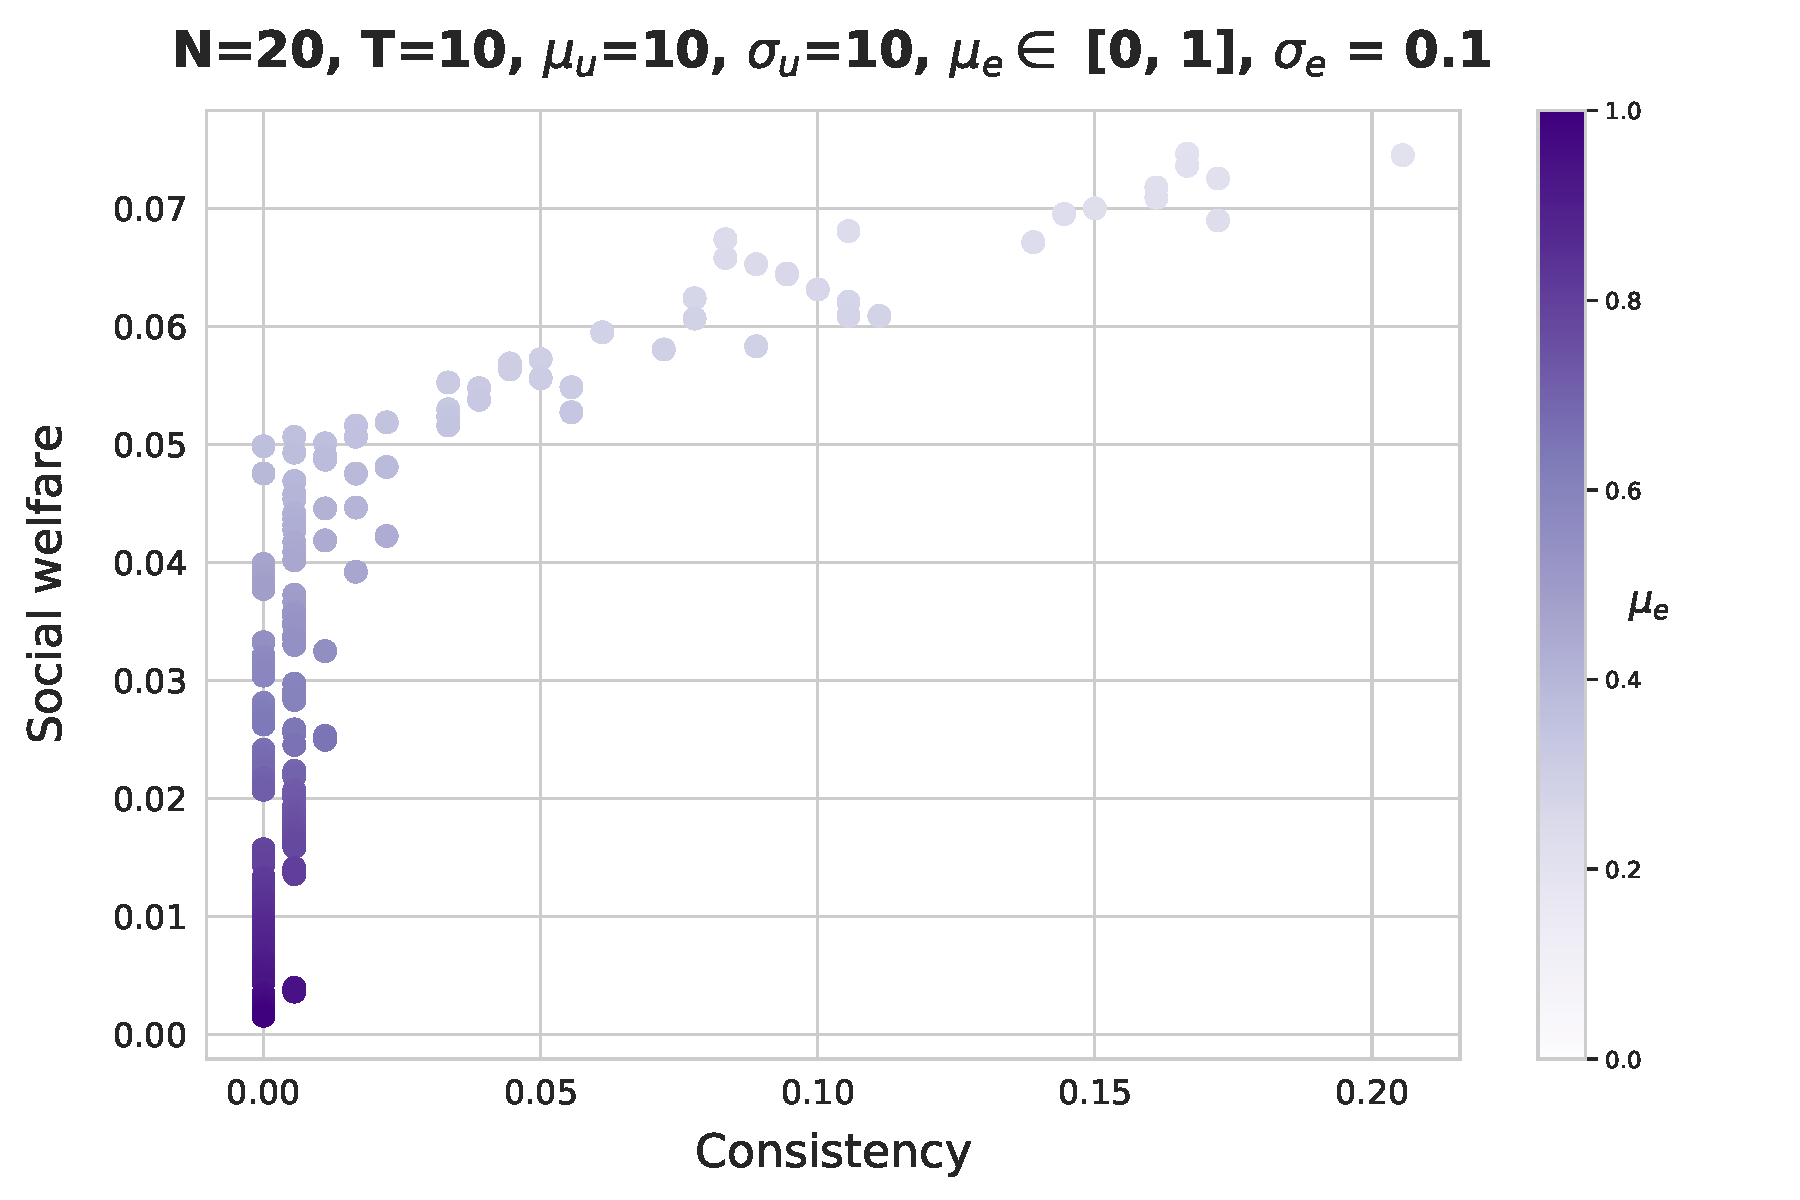
\includegraphics[width=0.32\linewidth]{figures/mpda_dynamics_excitement_mean.pdf}
     \caption{Mean social welfare vs. consistency for MPDA applied in various settings with 20 men/women and 10 time steps. (Left) Fixed excitement with varying utilities initialization (fixed mean). (Middle) Fixed utilities initialization but varying excitement (fixed mean) (b) fixed initialization varying excitement (fixed mean). (Right) Fixed utilities initialization but varying excitement (fixed variance).}
    \label{fig:mpda_dynamics}
\end{figure}
% \begin{figure}
%     \centering
%         \begin{subfigure}[b]{0.49\textwidth}
%          \centering
%          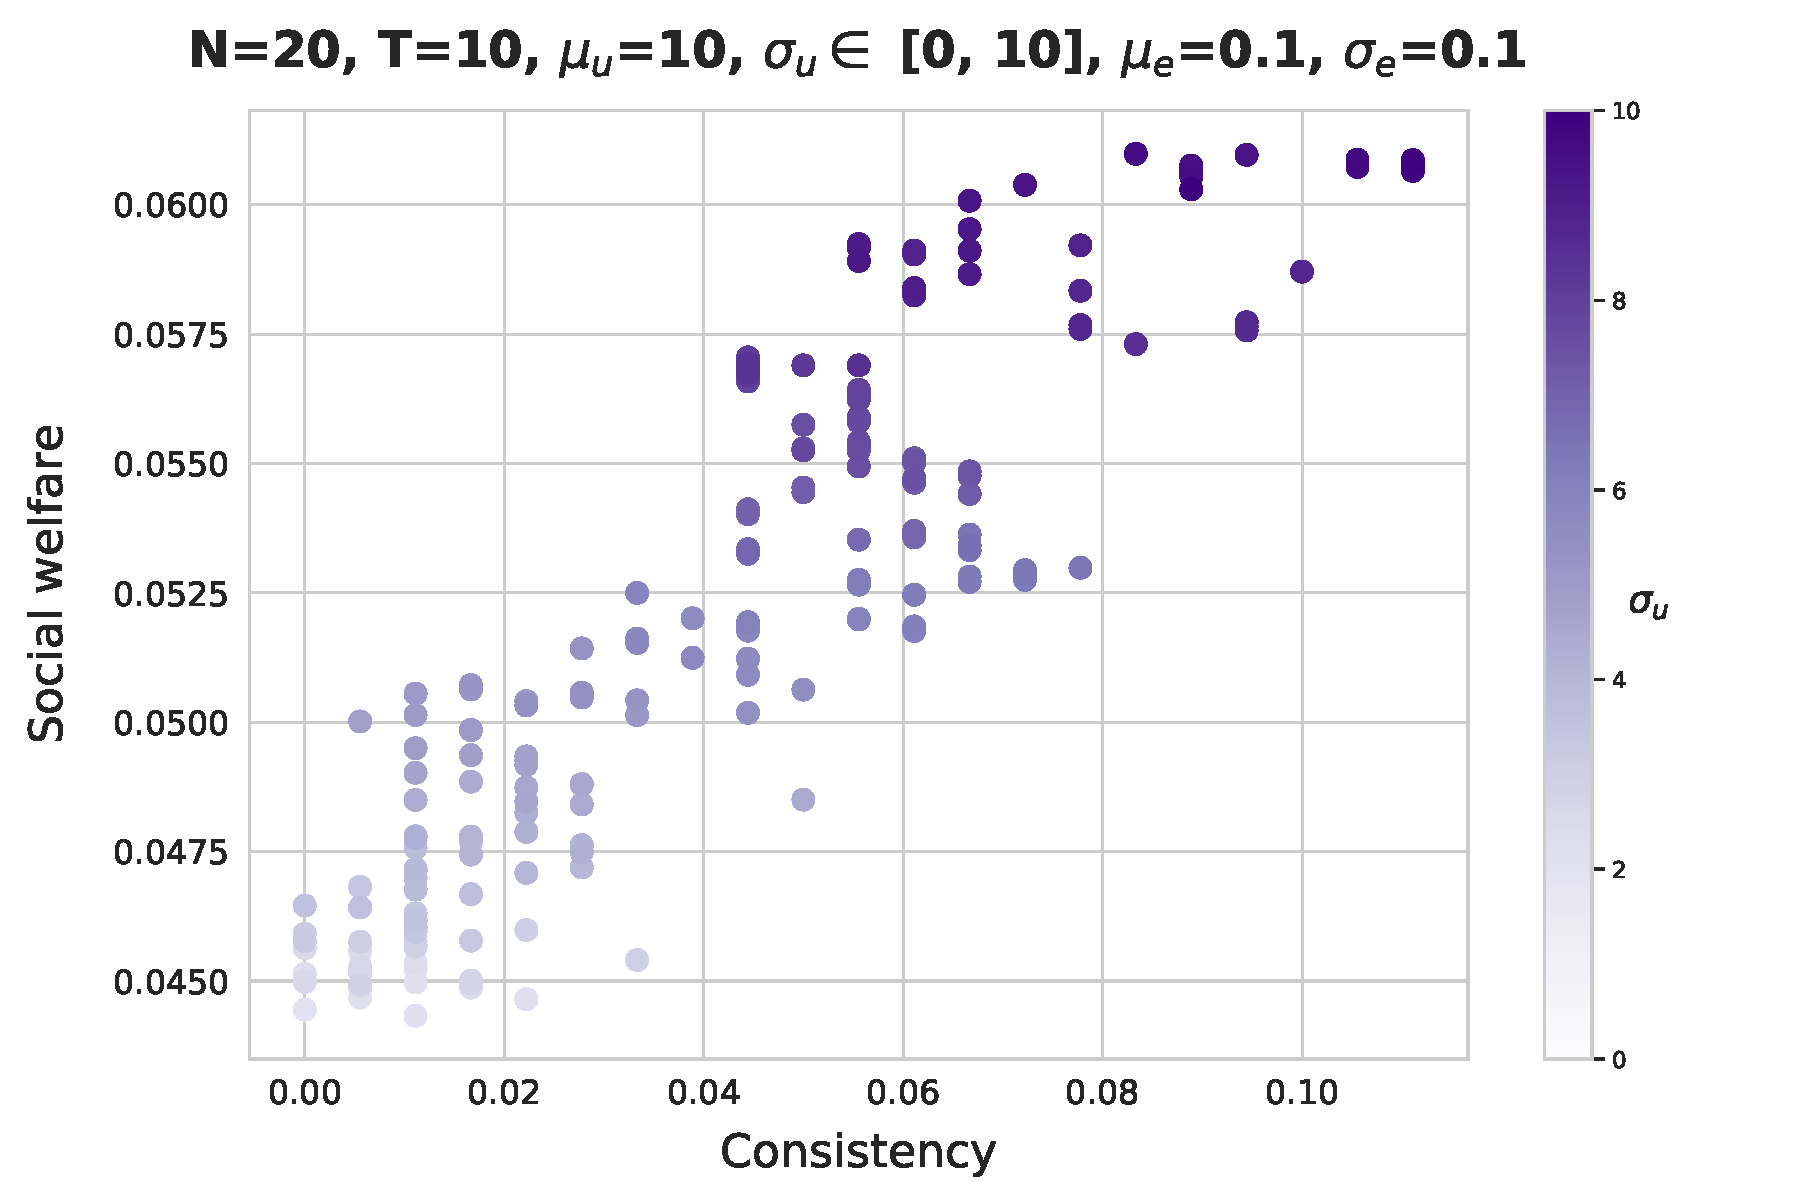
\includegraphics[width=\textwidth]{figures/mpda_dynamics_initliazation.pdf}
%          \caption{Dynamic Initialization}
%          \label{fig:init}
%         \end{subfigure}
%          \begin{subfigure}[b]{0.49\textwidth}
%          \centering
%          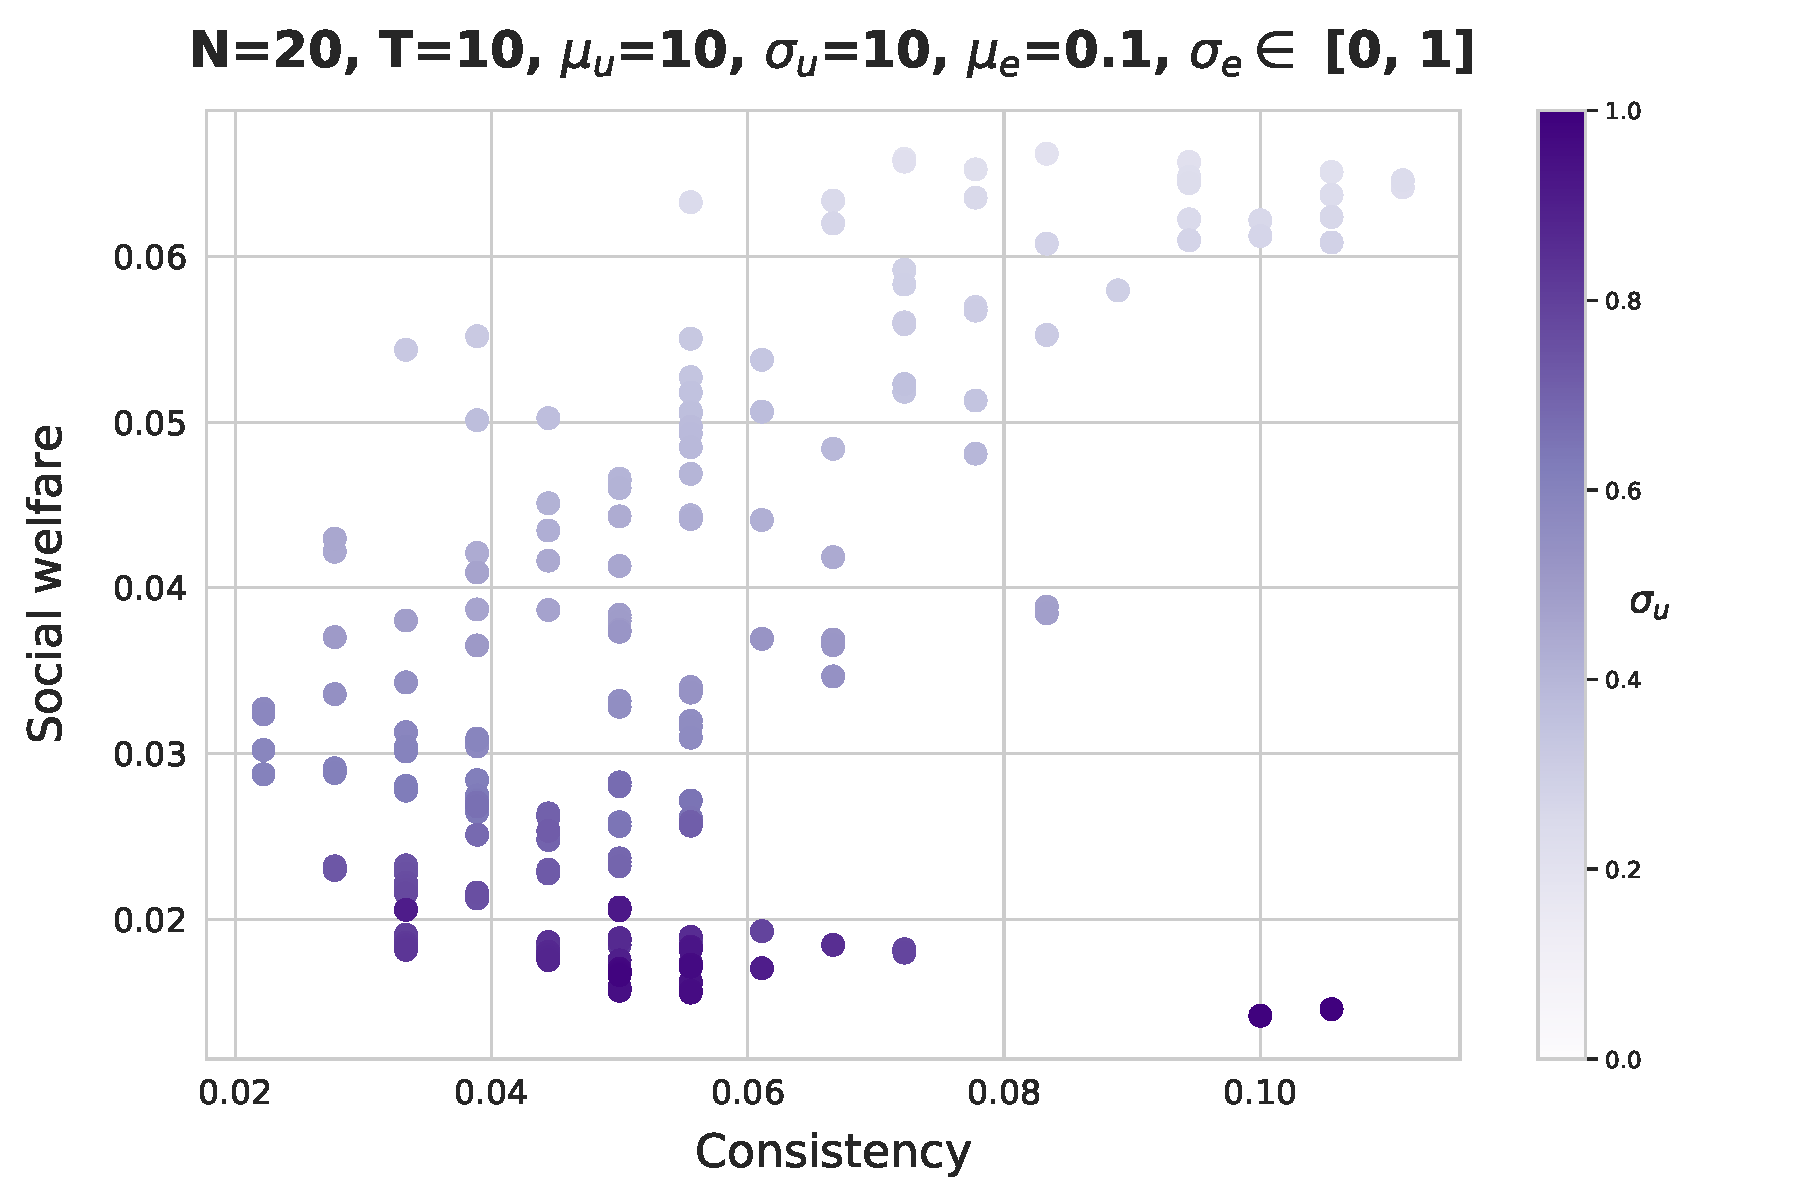
\includegraphics[width=\textwidth]{figures/mpda_dynamics_excitement_std.pdf}
%          \caption{Dynamic Excitement}
%          \label{fig:excite_std}
%      \end{subfigure}
%          \begin{subfigure}[b]{0.49\textwidth}
%          \centering
%          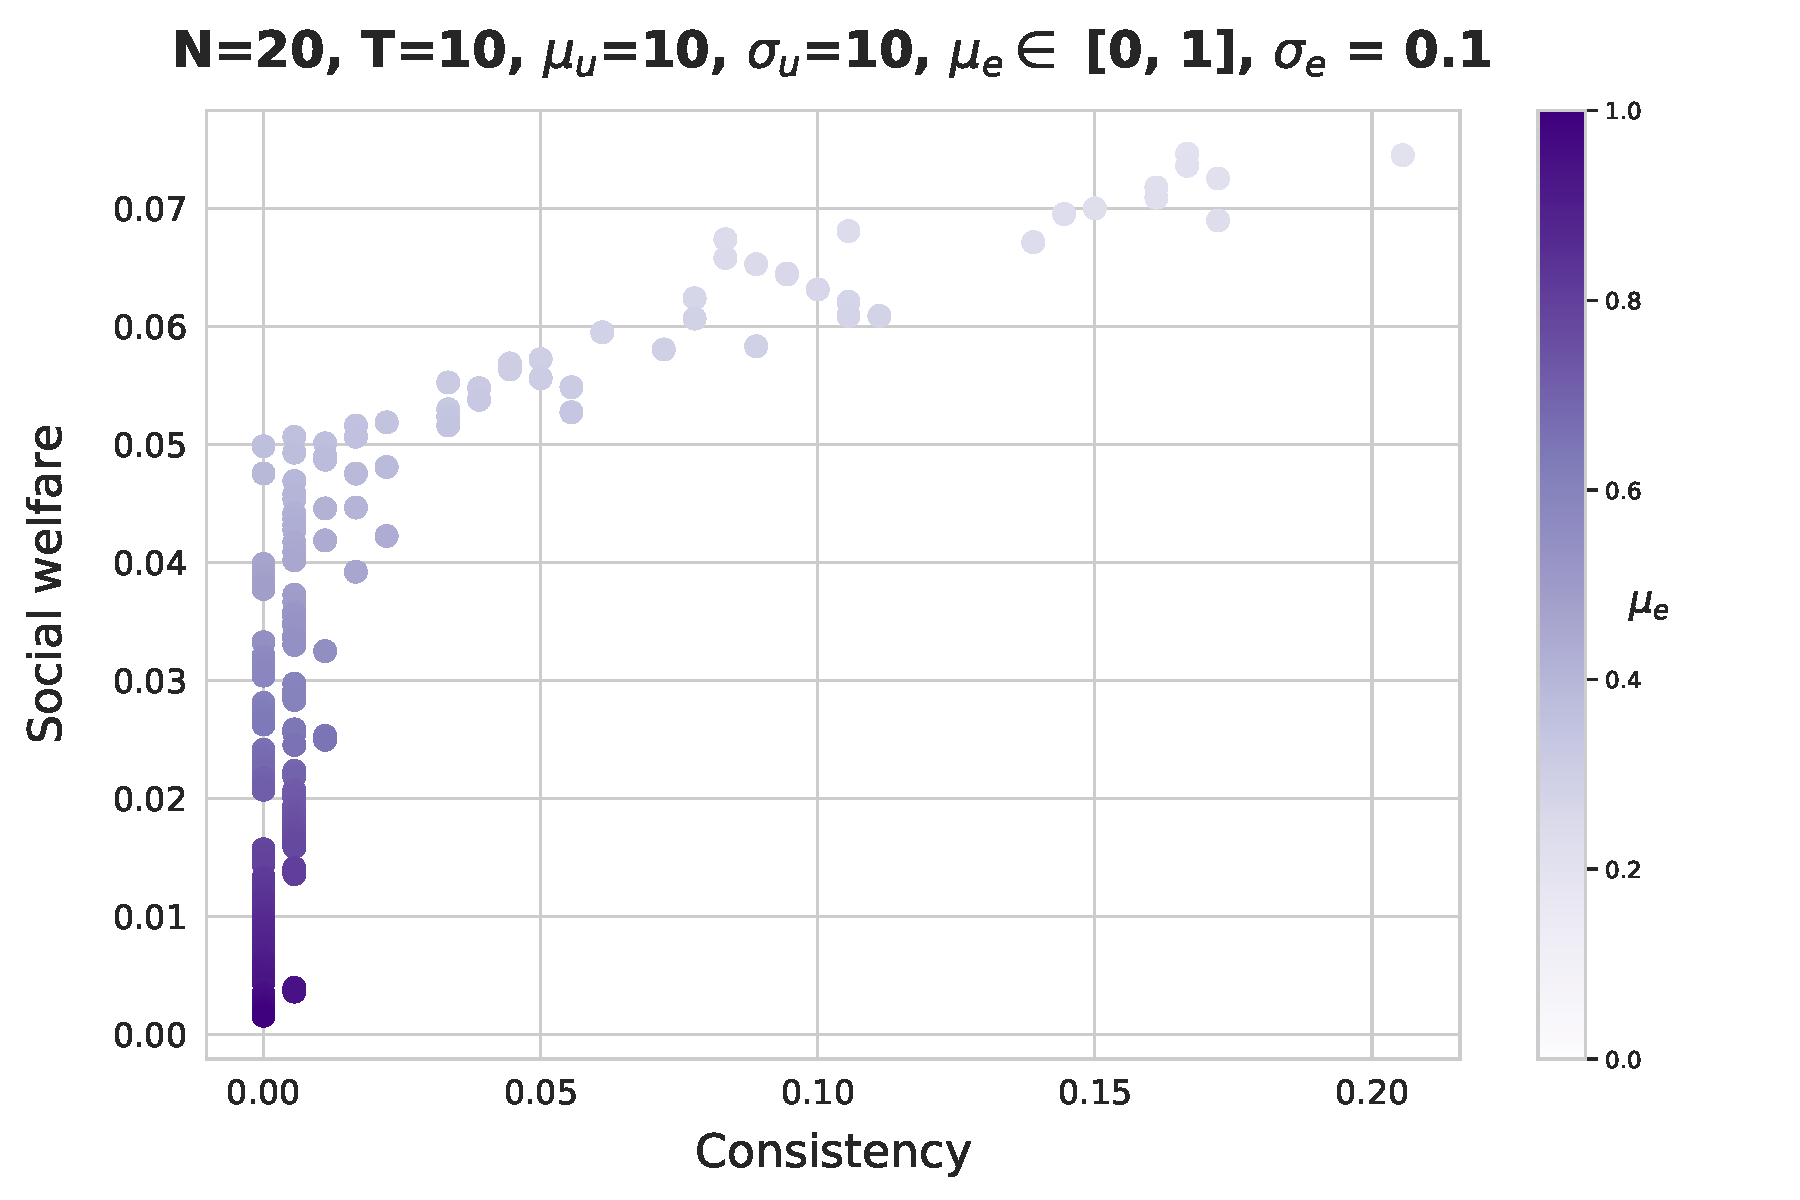
\includegraphics[width=\textwidth]{figures/mpda_dynamics_excitement_mean.pdf}
%          \caption{Dynamic Excitement}
%          \label{fig:excite_mean}
%      \end{subfigure}
%      \caption{Mean social welfare vs. consistency for MPDA applied to two dyanmic scenarios; (a) fixed excitement; (b) fixed initialization varying excitement (fixed mean); (c) fized initialization with varying excitement (fixed standard deviation).}
%     \label{fig:mpda_dynamics}
% \end{figure}

\paragraph{Dynamics} We first perform an ablation study with various utilities and excitement initializations. We run MPDA in a few dynamics settings with varying $\sigma_u$, $\mu_e$ and $\sigma_e$. Fig.~\ref{fig:mpda_dynamics} illustrates the results. Note that $\mu_u$ has little significant since the utilities are normalized, hence we did not experiment with varying $\mu_u$. The results show that with a larger $\sigma_u$ leads to both higher social welfare and consistency, most likely due to the fact that agents start out more loyal to their top choices and therefore it takes longer for the preference profile to shift. In addition, larger $\mu_e$ and $\sigma_e$ result in more dynamical changes to the utilities, which generally causes smaller social welfare and consistency.

\begin{figure}
    \centering
    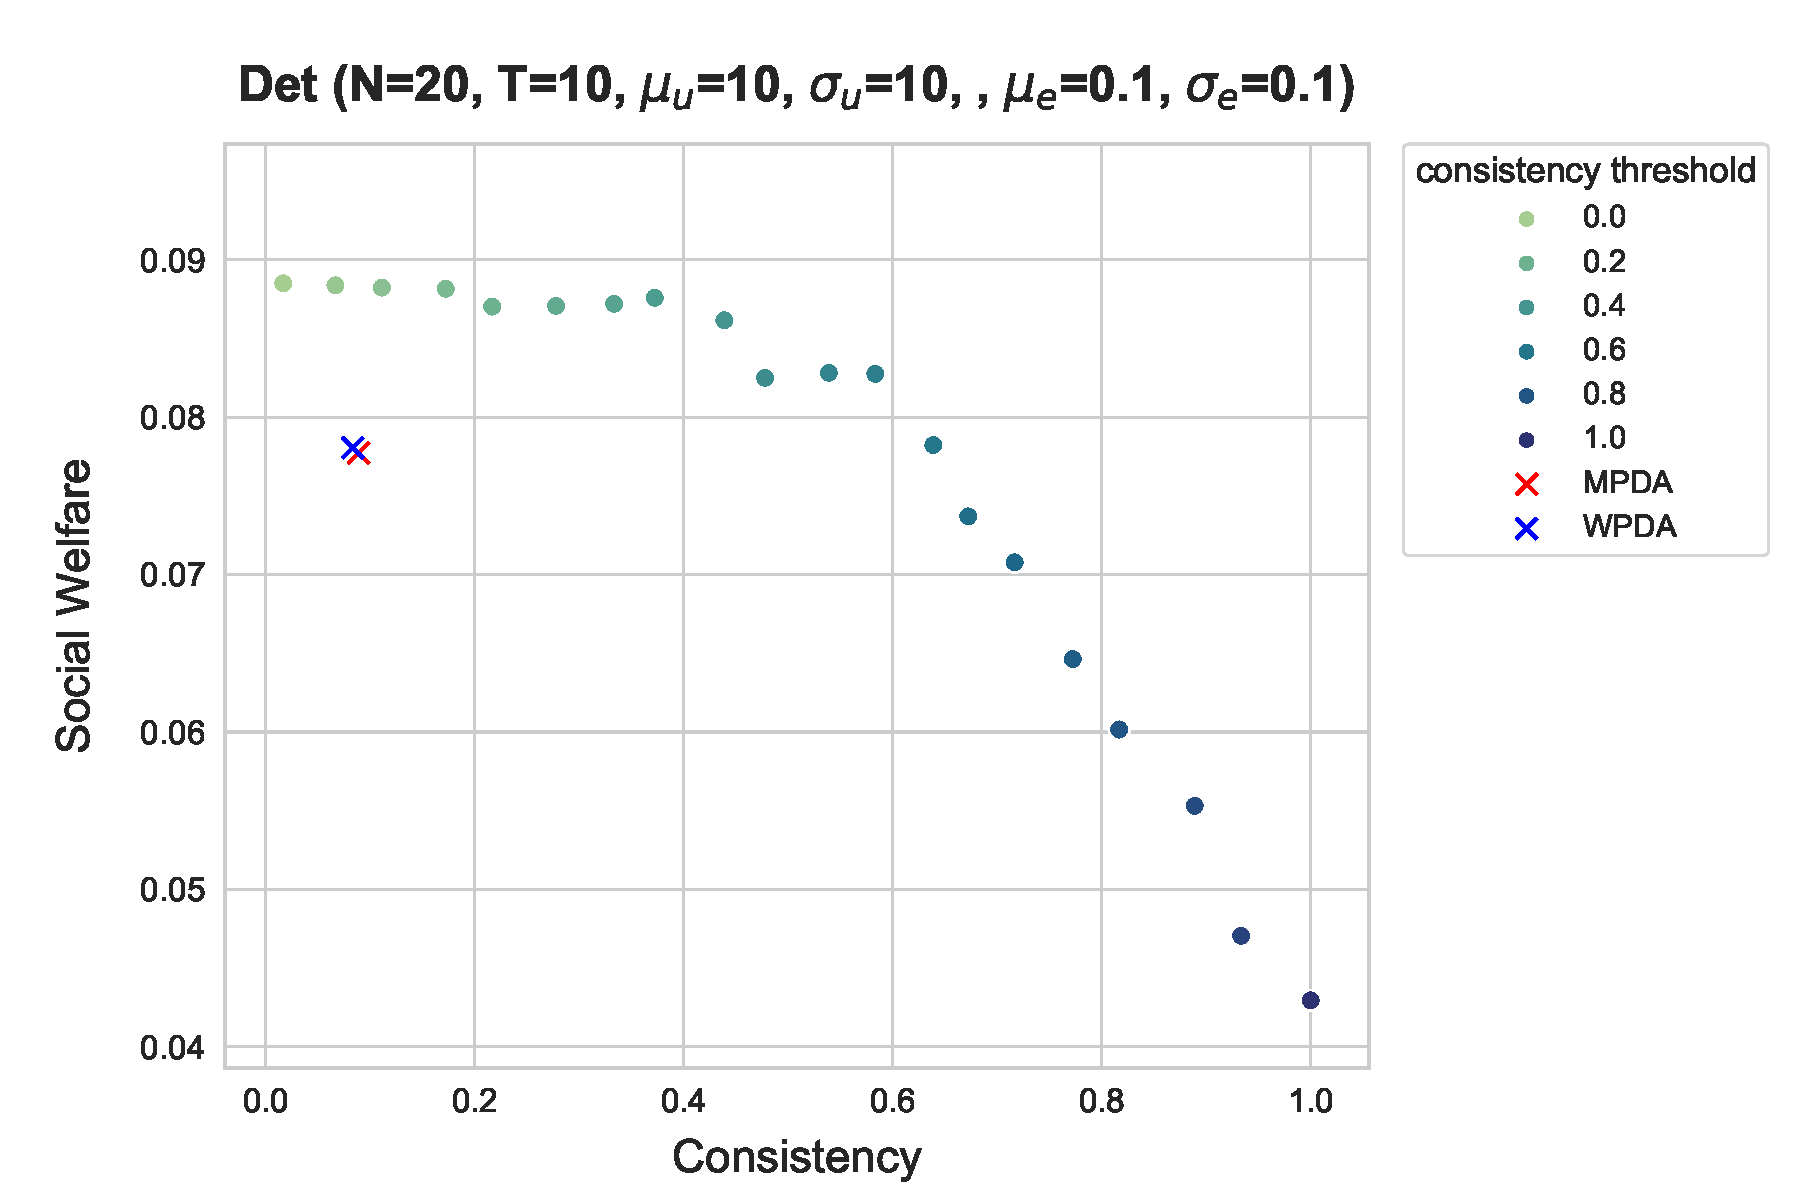
\includegraphics[width=0.32\linewidth]{figures/algs/Det_20_10_10_10.pdf}
    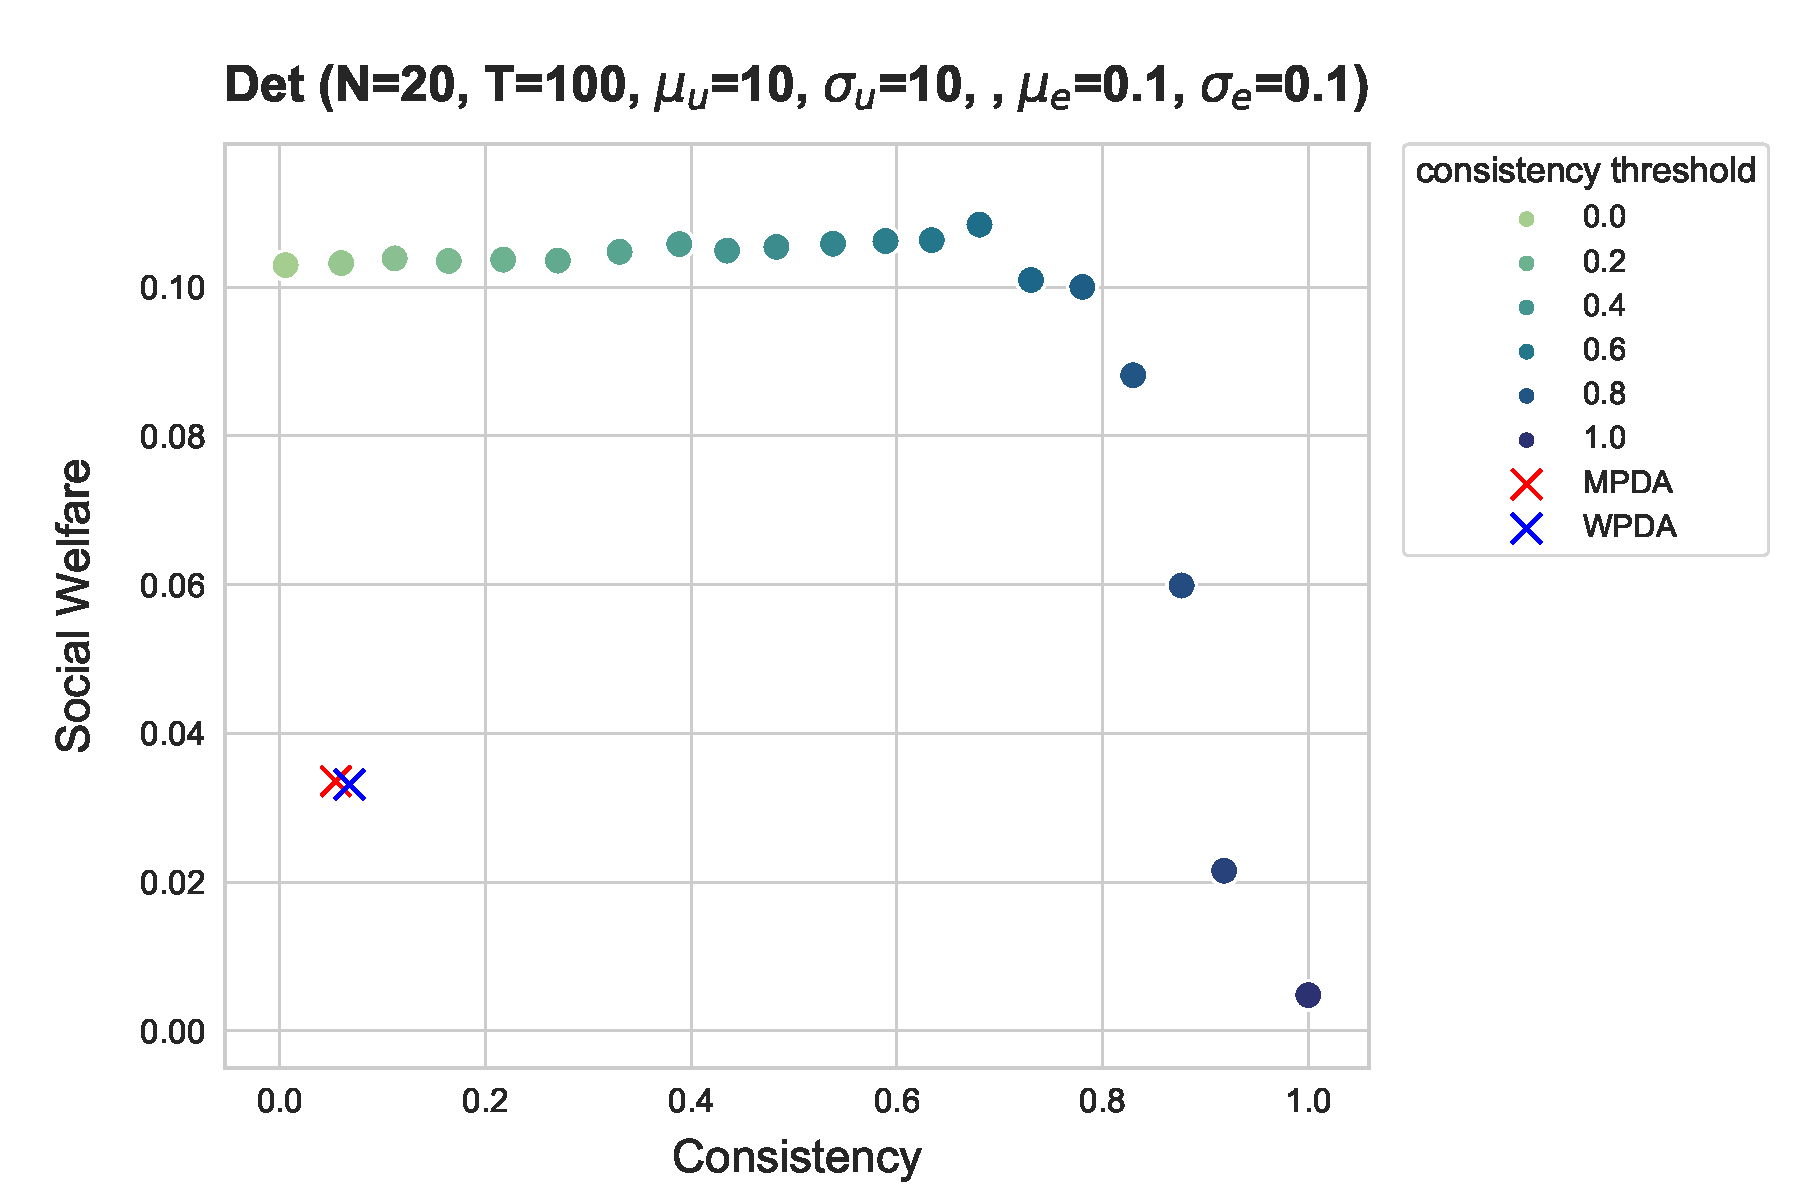
\includegraphics[width=0.32\linewidth]{figures/algs/Det_20_100_10_10.pdf}
    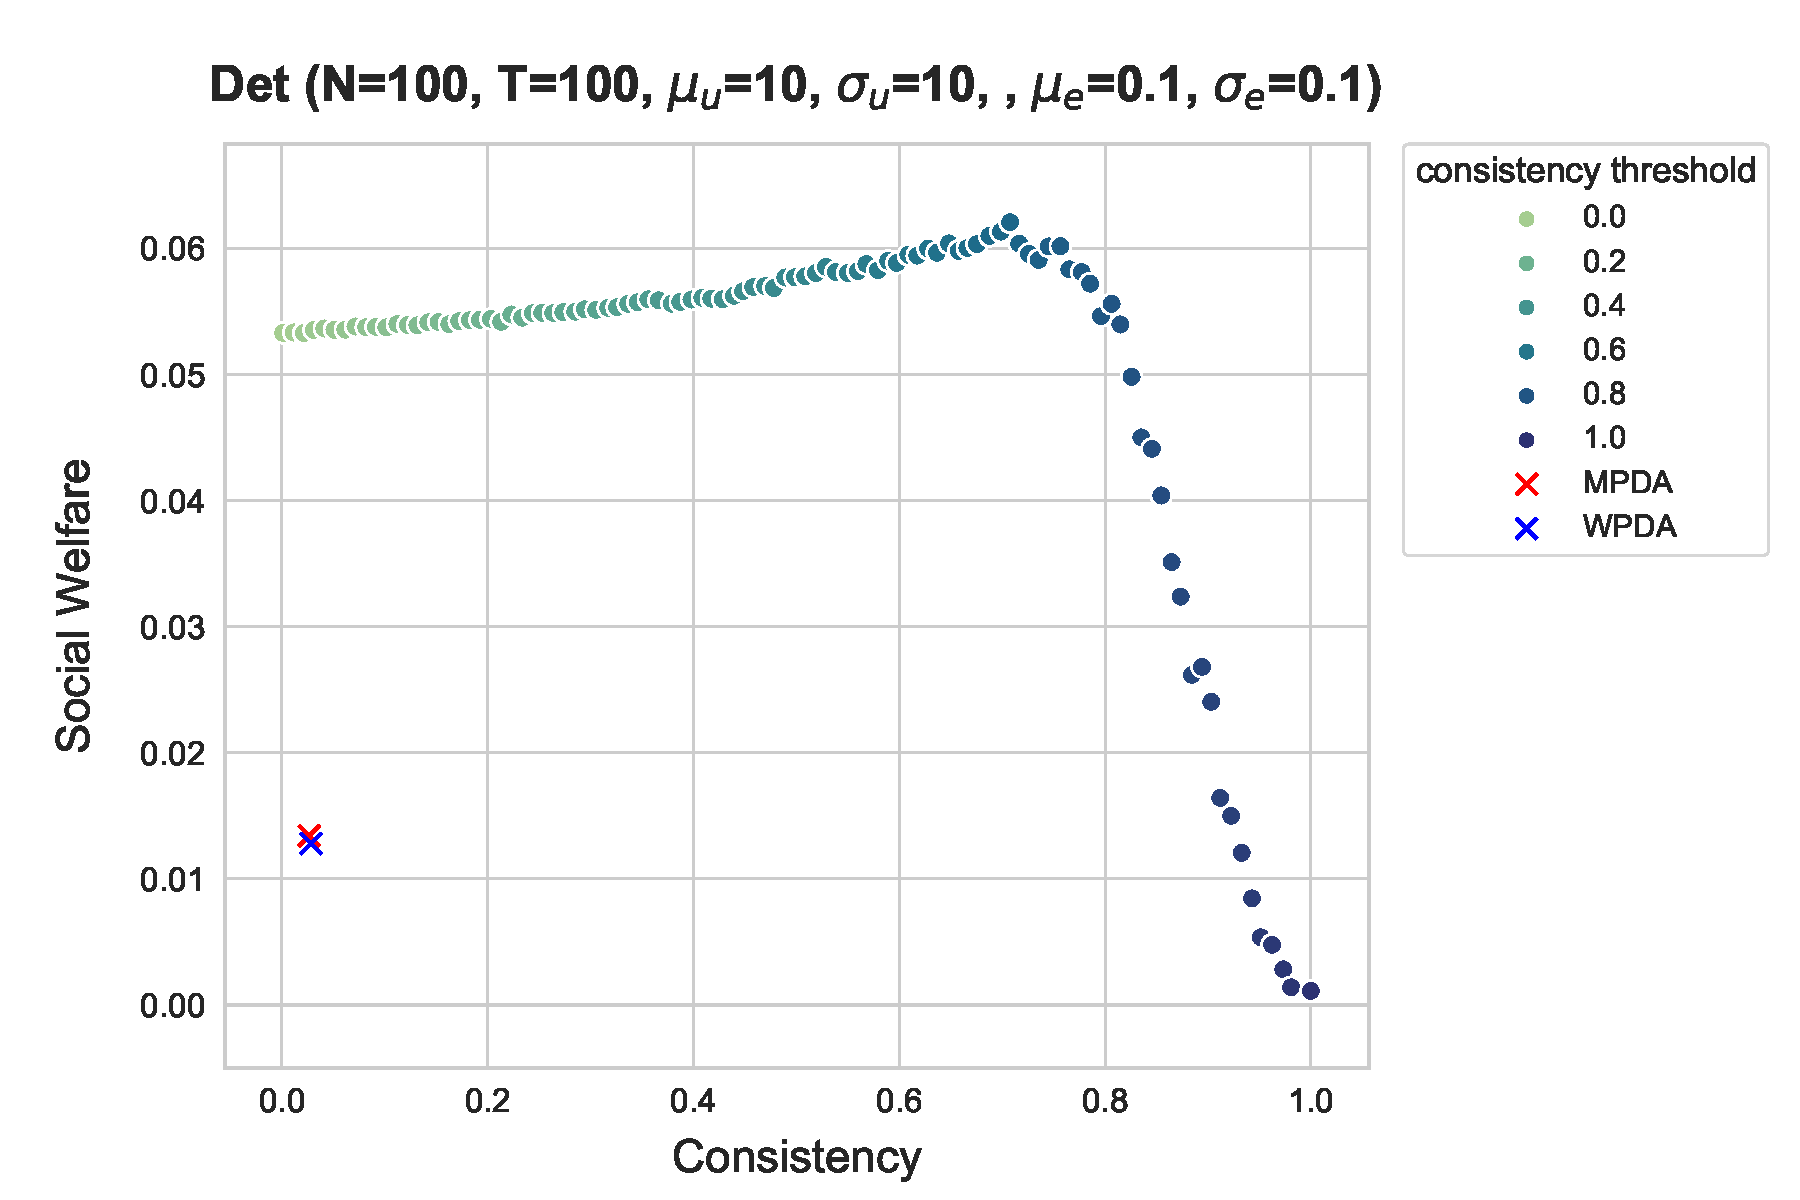
\includegraphics[width=0.32\linewidth]{figures/algs/Det_100_100_10_10.pdf}
    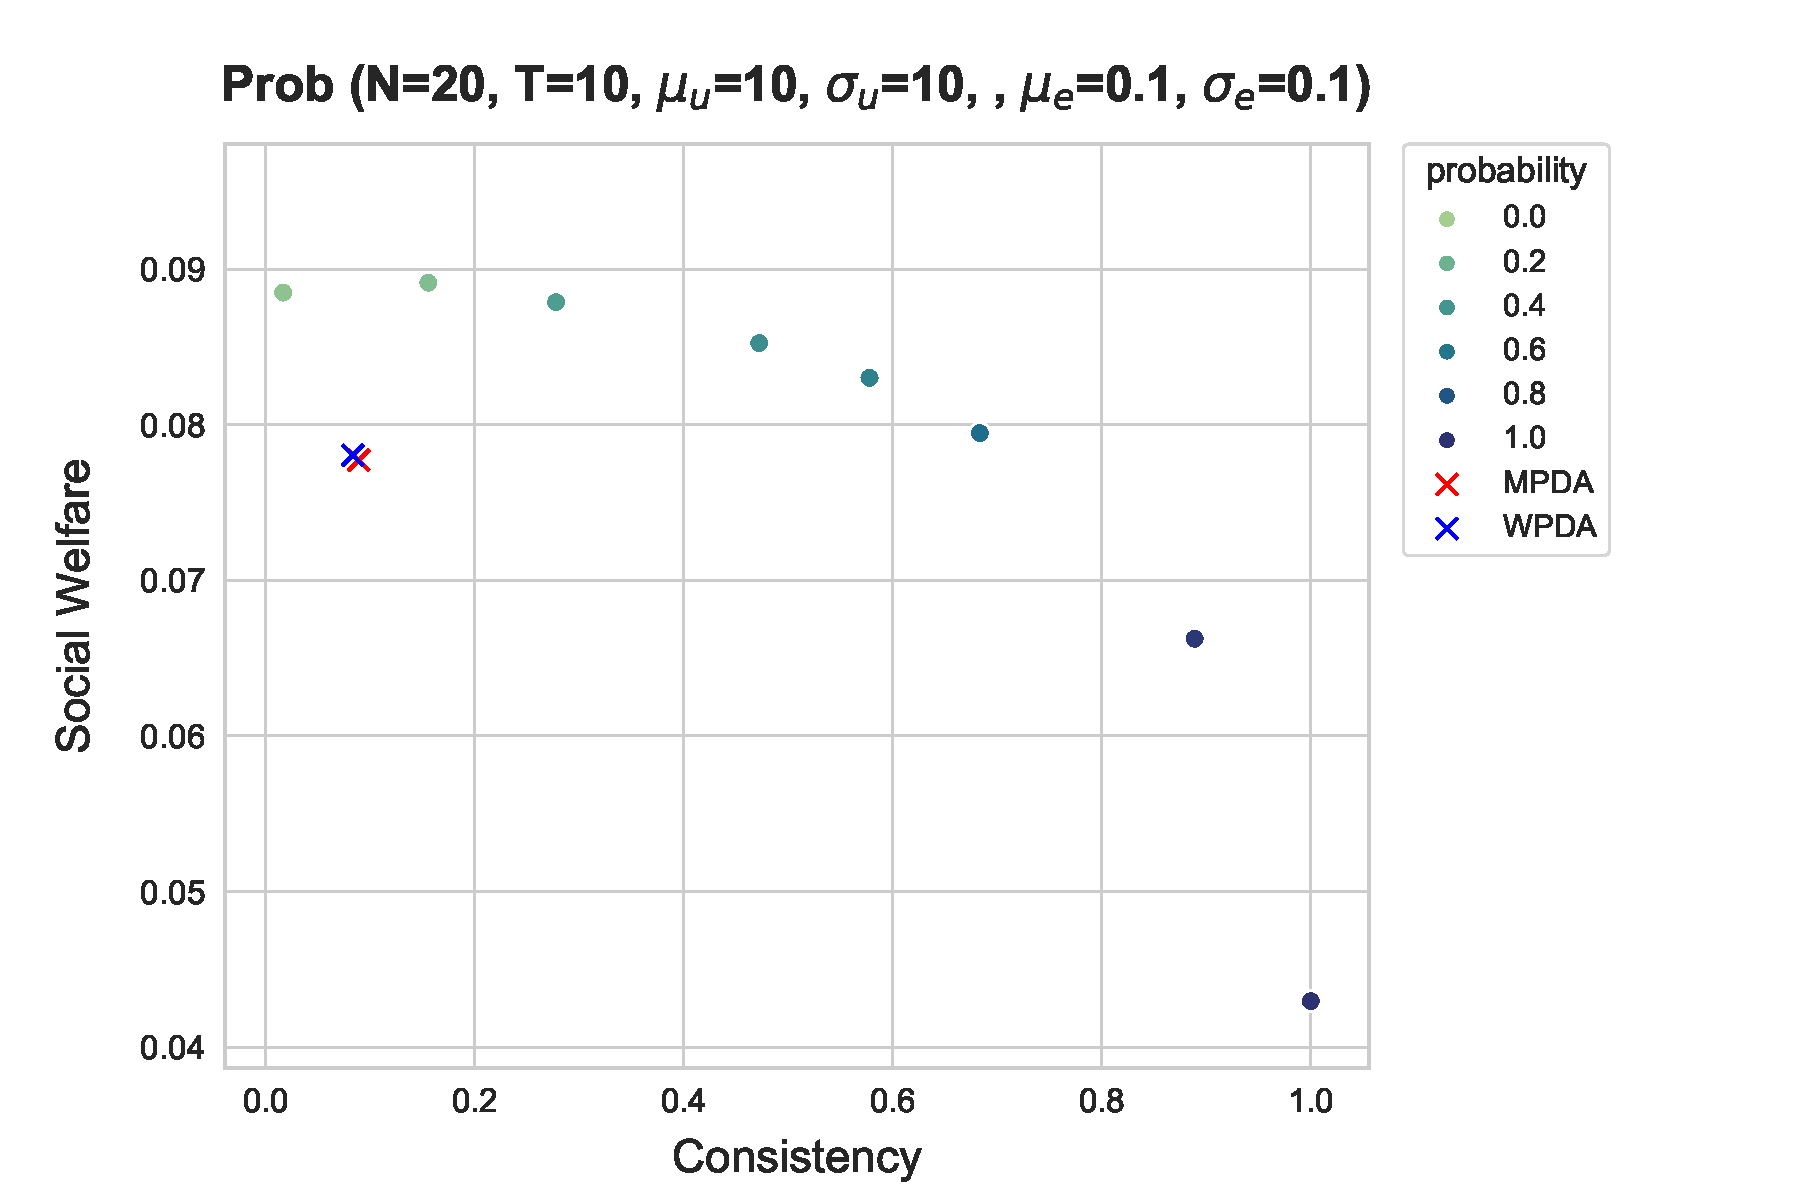
\includegraphics[width=0.32\linewidth]{figures/algs/Prob_20_10_10_10.pdf}
    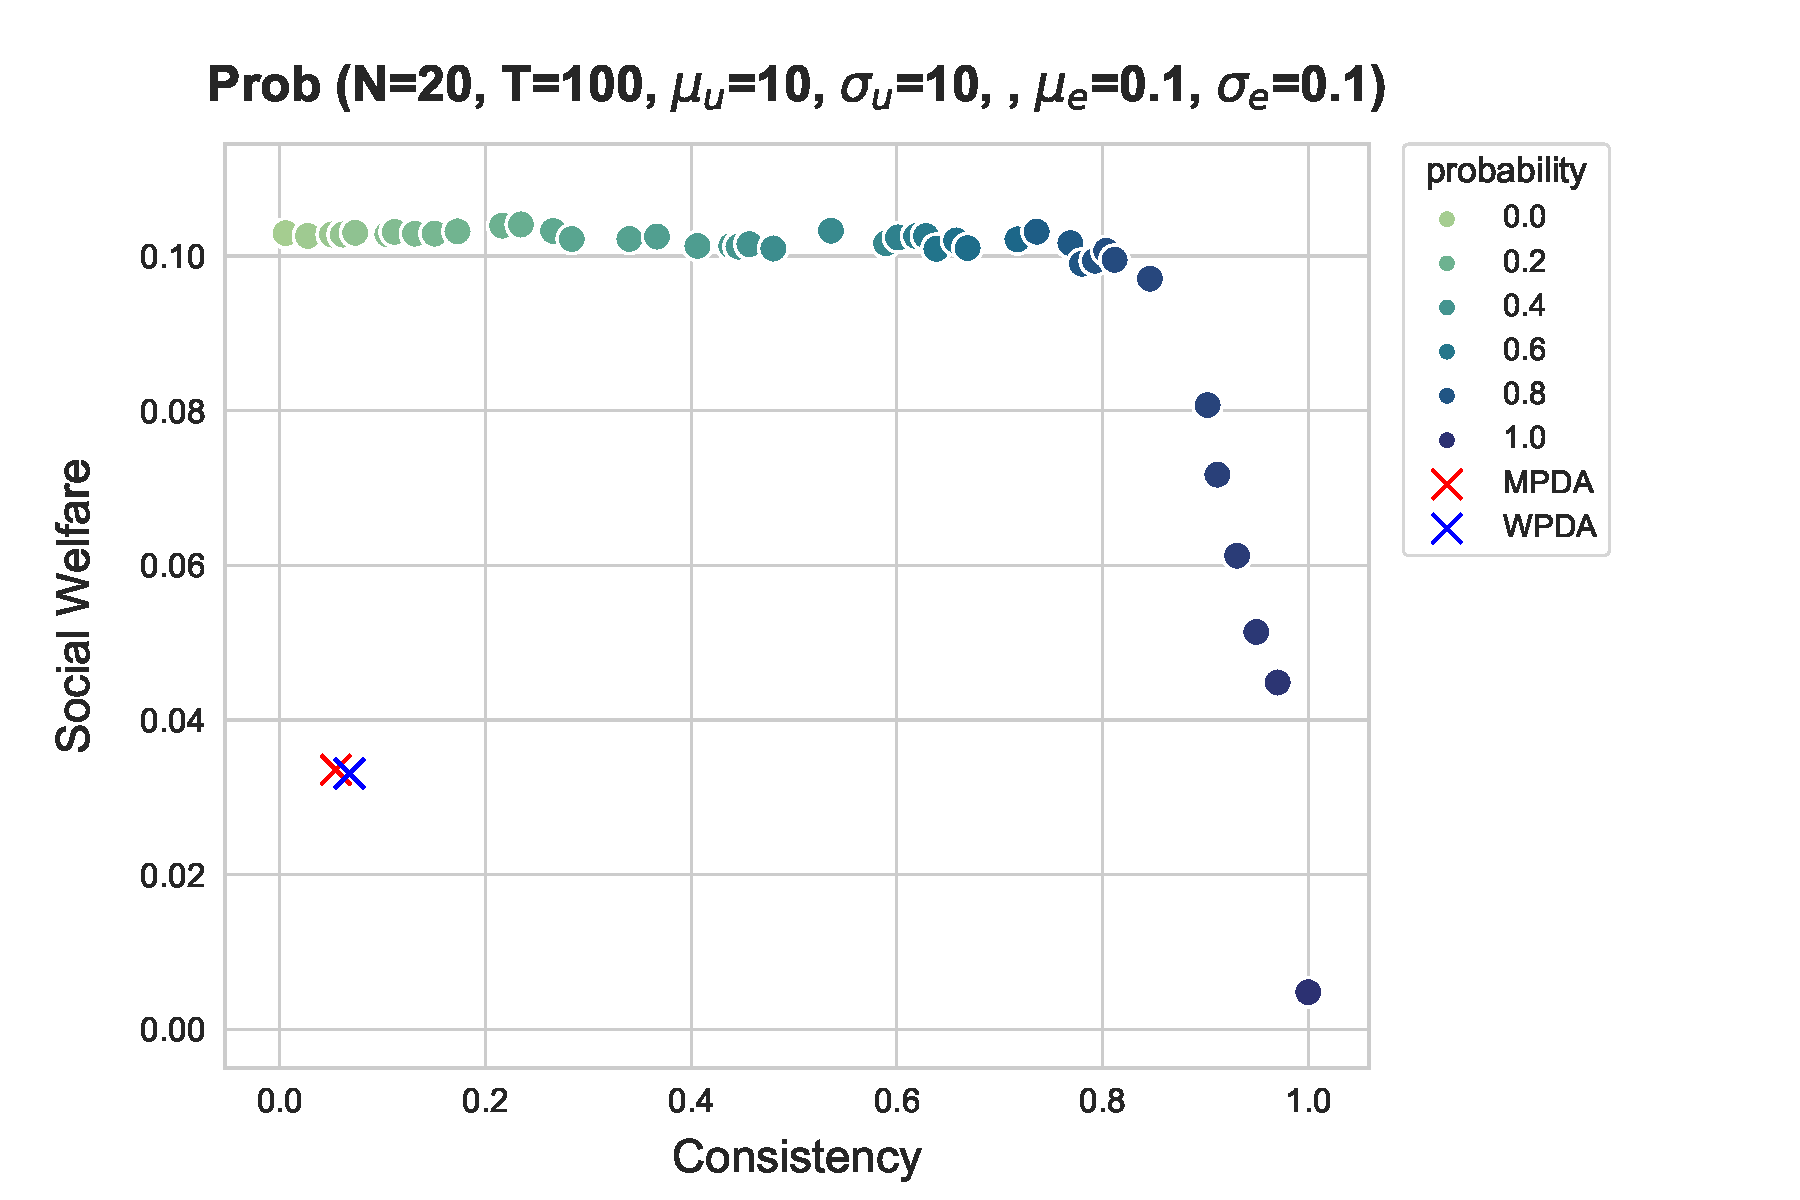
\includegraphics[width=0.32\linewidth]{figures/algs/Prob_20_100_10_10.pdf}
    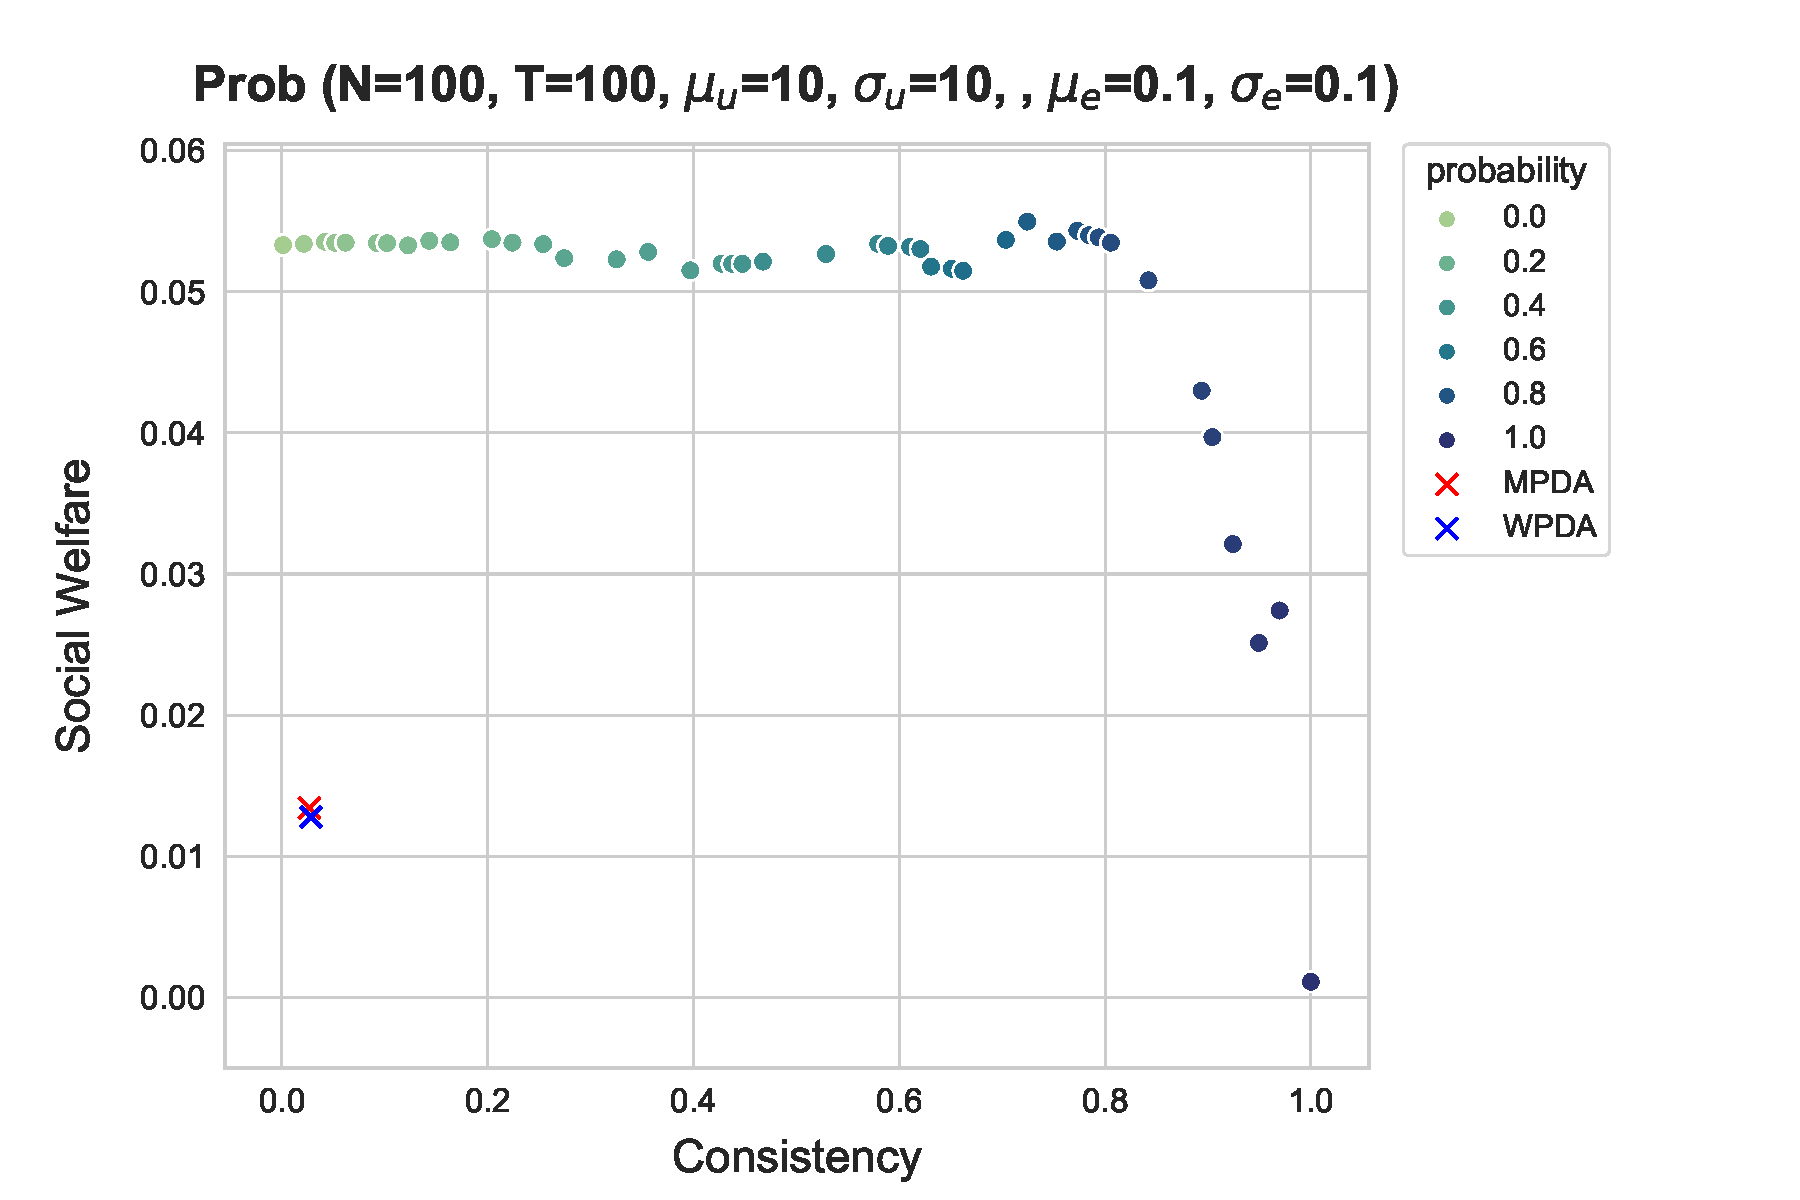
\includegraphics[width=0.32\linewidth]{figures/algs/Prob_100_100_10_10.pdf}
    \caption{Det (top row) and Prob (bottom row) algorithms in the setting where utilities are initialized with $\mathcal{N}(10, 10^2)$ and excitements are initialized with $\mathcal{N}(0.1, 0.1^2)$, with 20 agents and 10 time steps (left column), 20 agents and 100 time steps (middle column), and 100 agents and 100 time steps (right column) respectively.}
    \label{fig:algs}
\end{figure}
\begin{wrapfigure}{R}{0.3\textwidth}
     \vspace{-7mm}
        \centering
        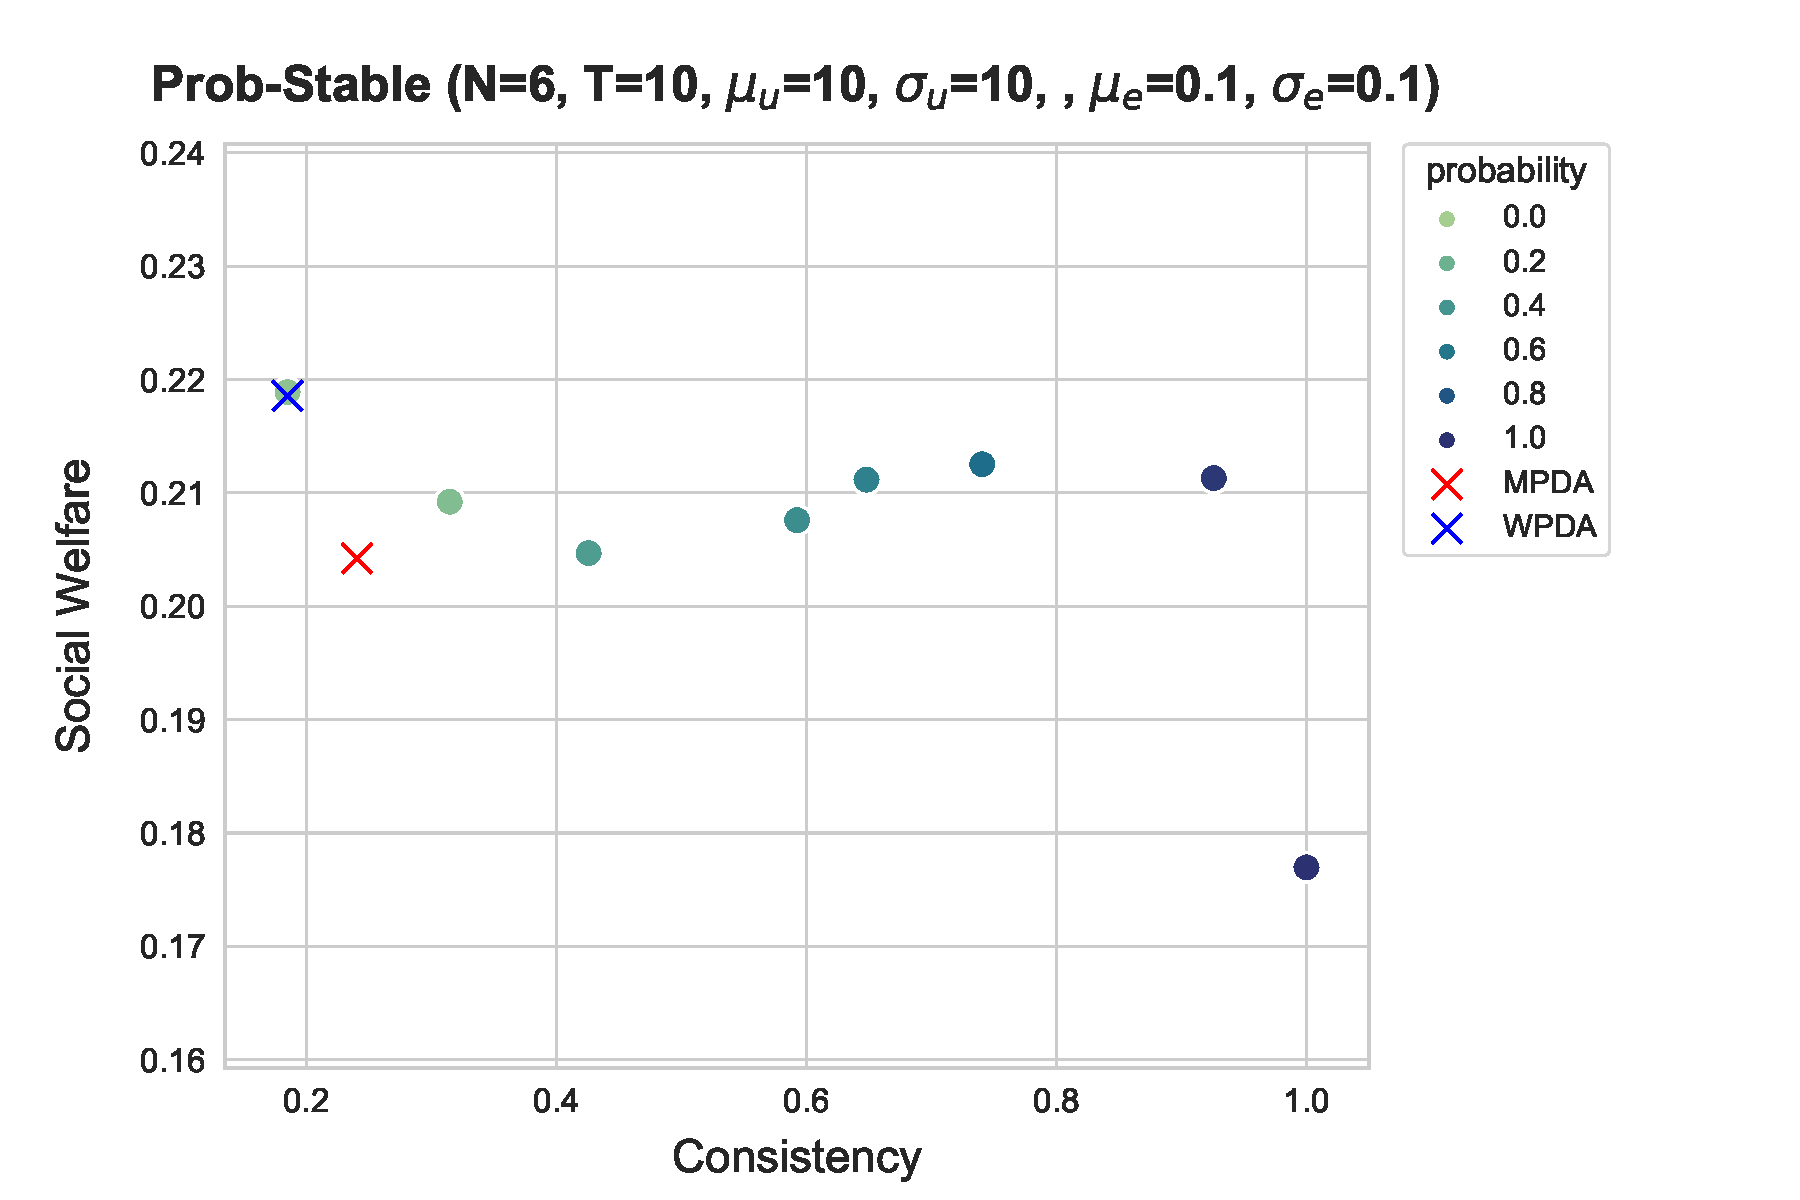
\includegraphics[width=0.3\textwidth]{figures/algs/Prob-Stable_6_10_10_10.pdf}
        \caption{Prob-Stable for $N=6$ and $T=10$.
        \label{fig:prob-stable}}
     \vspace{-15mm}
\end{wrapfigure}

\paragraph{Algorithms} We next run MPDA, WPDA, Det, Prob and Prob-Stable in the dynamics setting with $\mu_u = \sigma_u = 10$ and $\mu_e = \sigma_e = 0.1$. We choose this setting since the initialized utilities are diverse and the excitements are not too drastic. We experiment with $(N=20, T=10)$, $(N=20, T=100)$ and $(N=100, T=100)$ respectively. Fig.~\ref{fig:algs} showcases the results of Det and Prob compared to MPDA and WPDA. For both Det and Prob, we see that a higher threshold of $c$ or $p$, which constrains the results to have a higher consistency, generally leads to smaller social welfare. Nevertheless, we observe that with $T=100$ total time steps, the social welfare peaks at around 0.6 consistency, which shows that putting a constraint on the marriage consistency leads to better long-term average social welfare than allowing agents to marry greedily according to their utilities at every time step. Furthermore, we show that with more agents and longer time horizon, the performance gap between MPDA/WPDA and Det/Prob increases in terms of both consistency and social welfare. This is likely due to the fact that with more agents and more time steps, it is harder for a matching to stay stable and achieve maximum social welfare. A perhaps more fair comparison is shown in Fig.~\ref{fig:prob-stable} with the Prob-Stable algorithm, where WPDA has a closer performance as Prob-Stable with $p=0$.

\begin{figure}
    \centering
    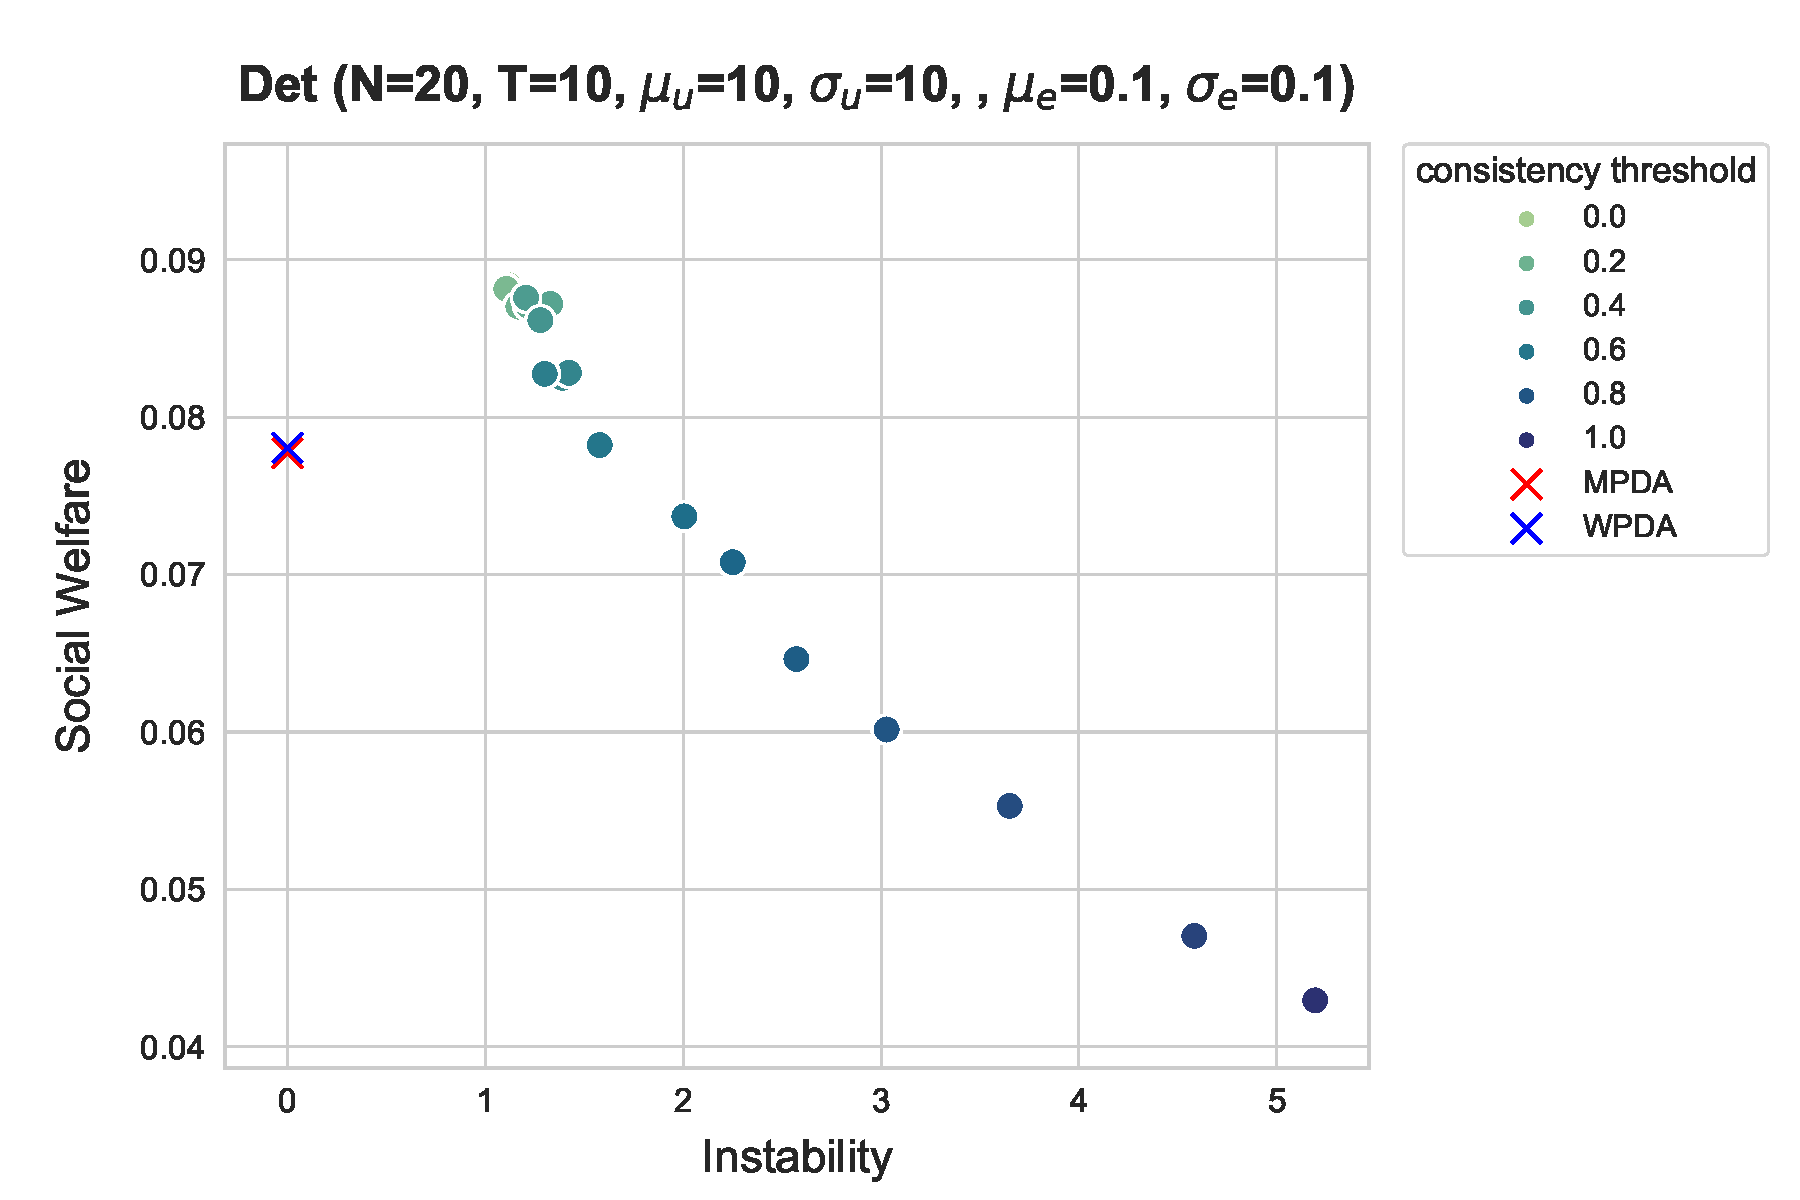
\includegraphics[width=0.32\linewidth]{figures/algs/Det_sw_20_10_10_10.pdf}
    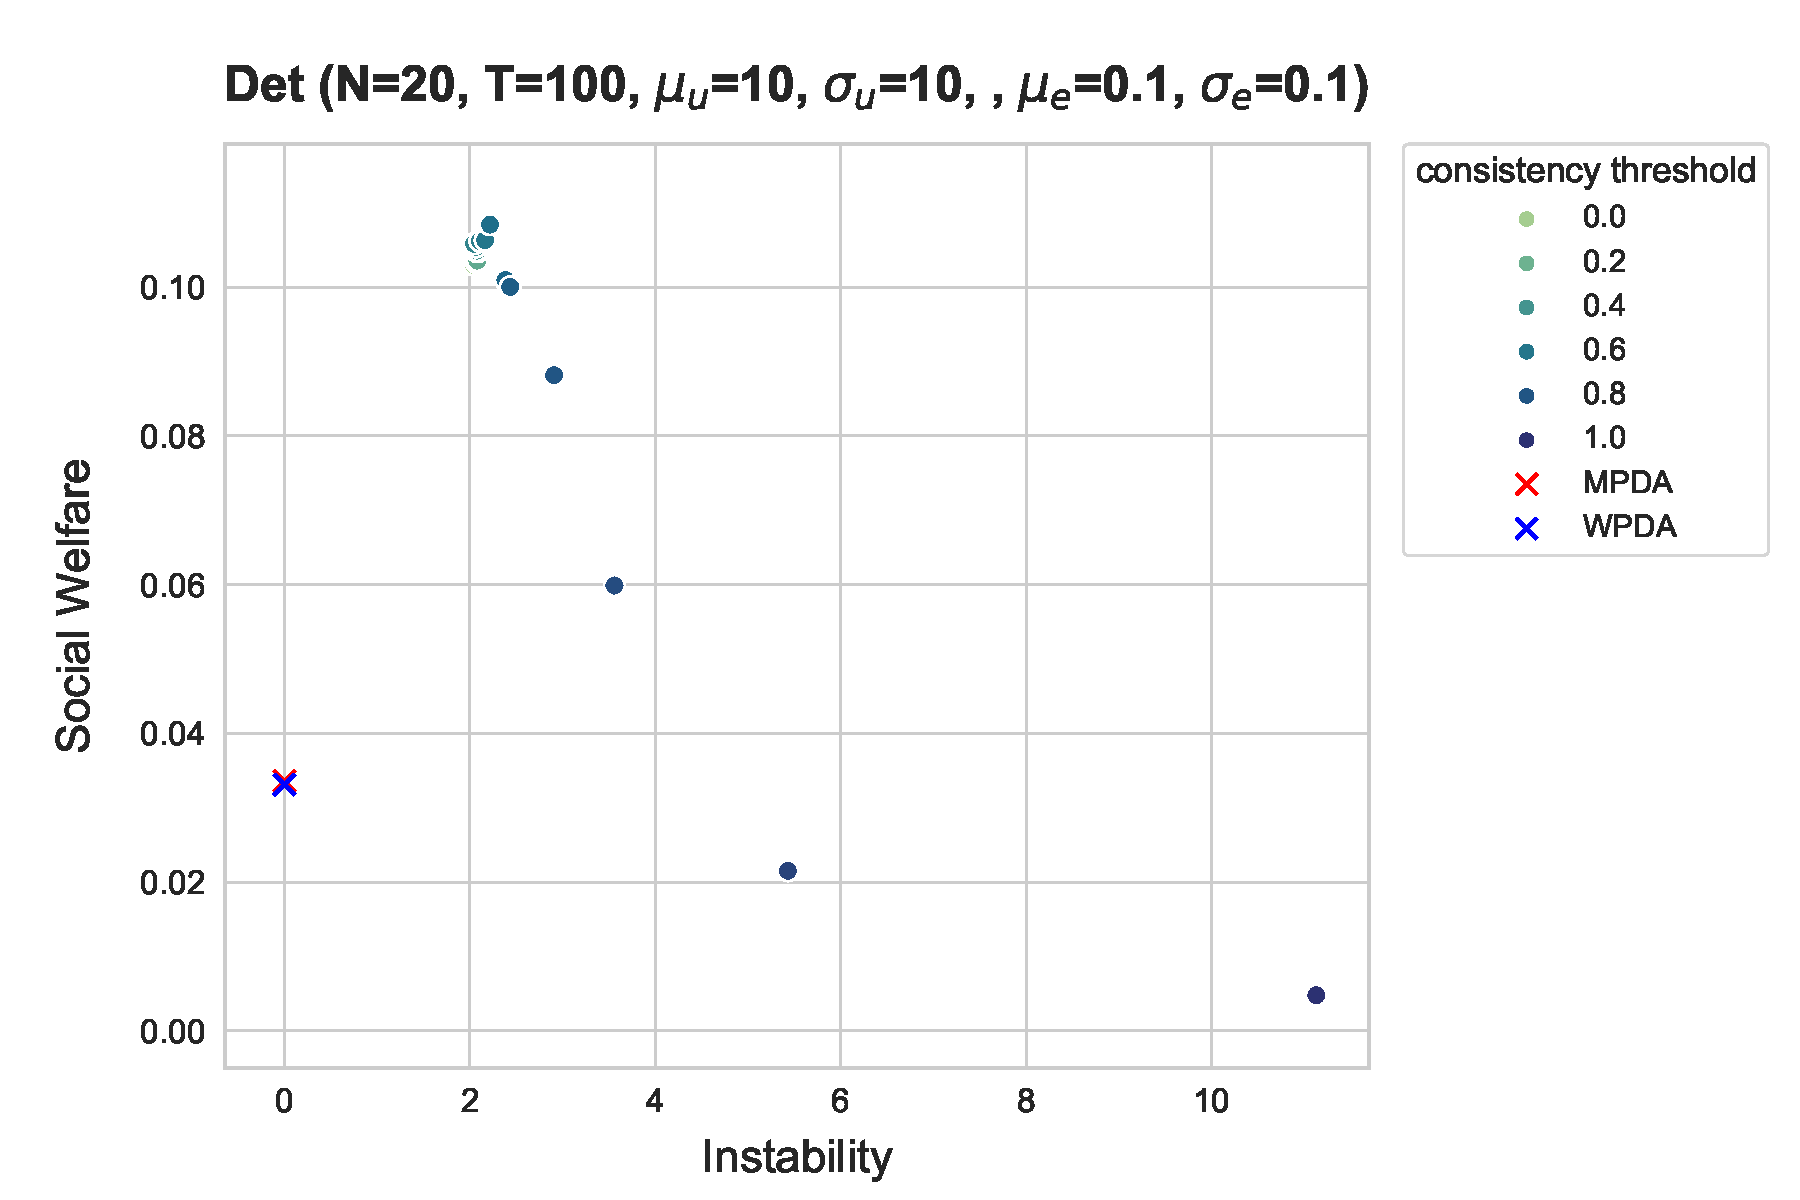
\includegraphics[width=0.32\linewidth]{figures/algs/Det_sw_20_100_10_10.pdf}
    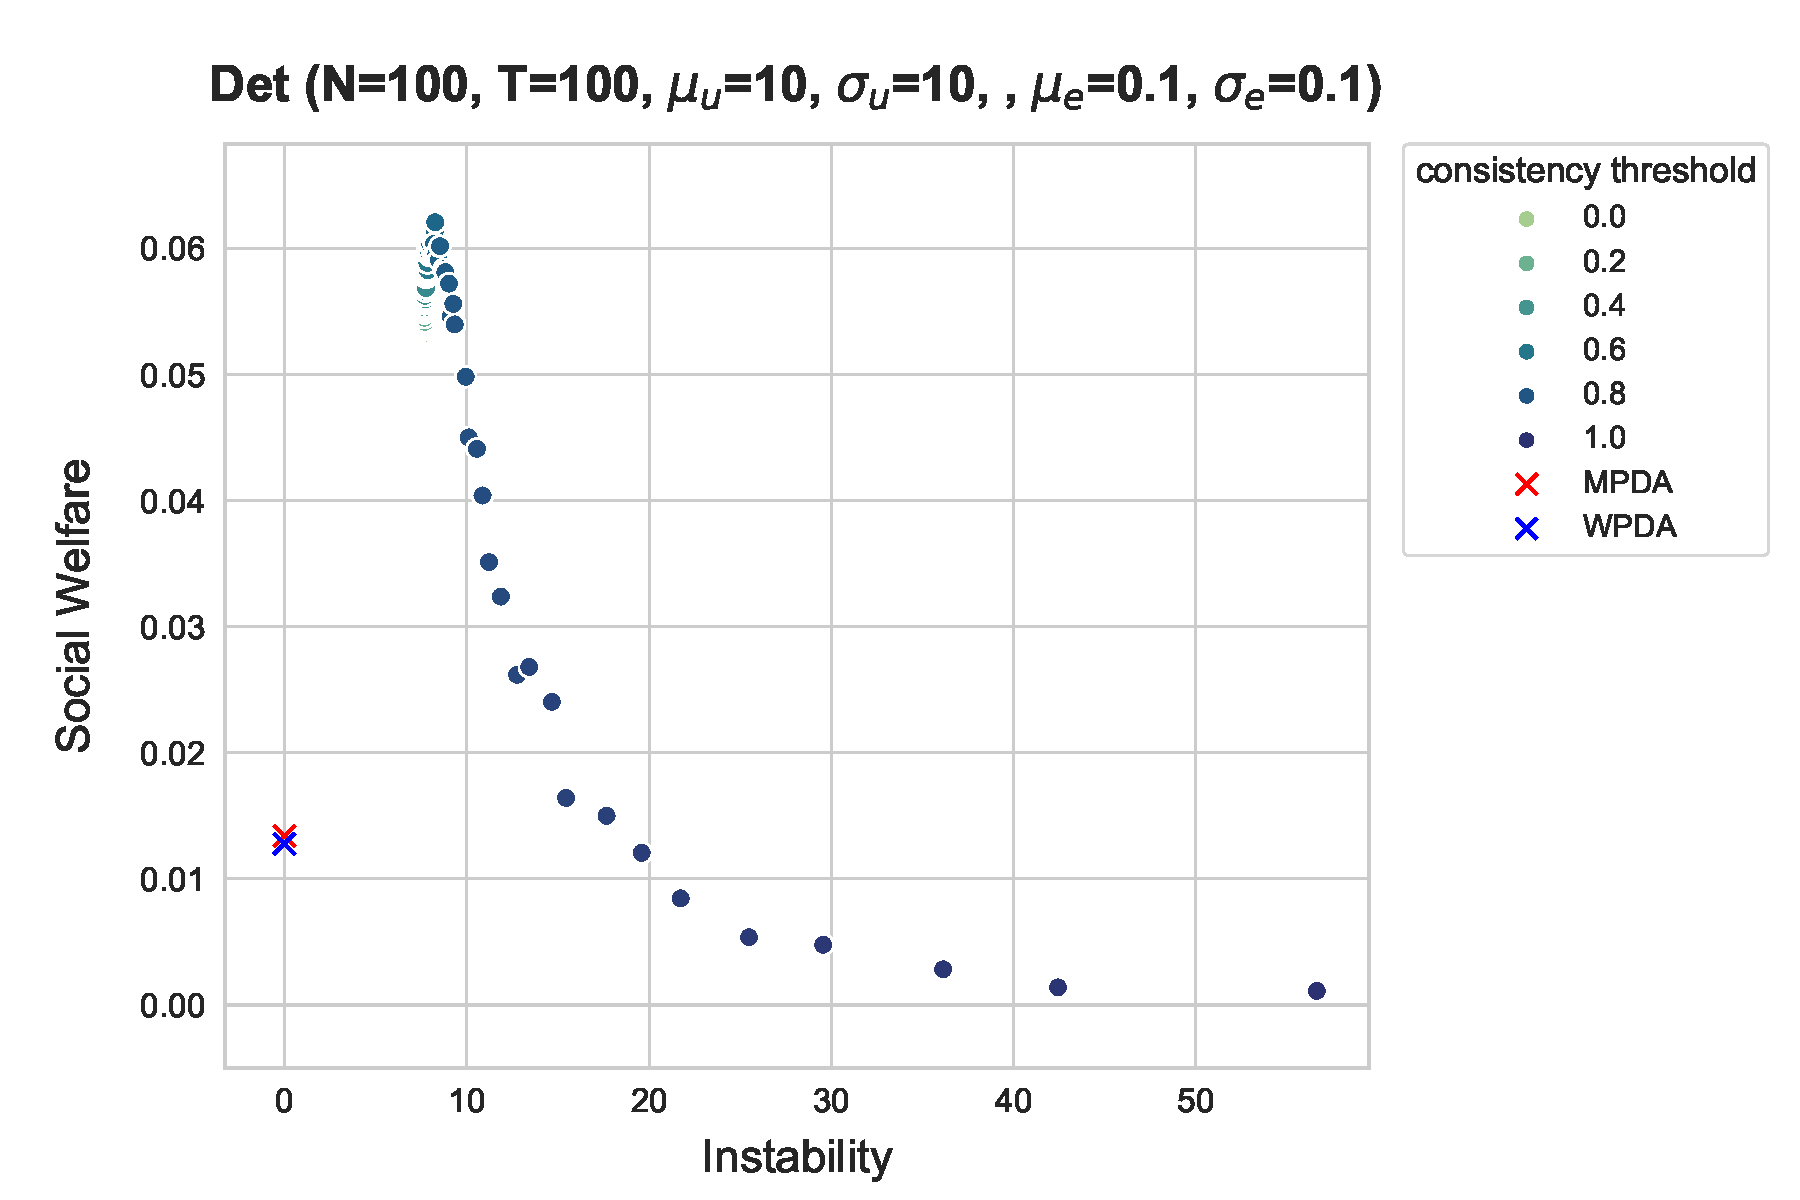
\includegraphics[width=0.32\linewidth]{figures/algs/Det_sw_100_100_10_10.pdf}
    \caption{Instability vs. social welfare for Det vs. MPDA vs. WPDA, with 20 men/women and 10 time steps (left), 20 men/women and 100 time steps (middle), and 100 men/women and 100 time steps (right).}
    \label{fig:det-stability}
\end{figure}
\paragraph{Stability vs. Social Welfare} We also evaluate the stability of Det. Fig.~\ref{fig:det-stability} shows that high social welfare is generally correlated with low instability. However, matching with maximum social welfare is still unstable, and a stable matching can have a much lower social welfare compared to the maximum.
% 0.5 - 1 page
% Figures and analysis
% \begin{itemize}
%     \item Evaluation of the algorithms (trade-off plot)
%     \begin{itemize}
%         \item scatter plot for the algorithm family
%         \item variance plot for the algorithm family
%     \end{itemize}
%     \item Evaluation with various dynamics
%     \begin{itemize}
%         \item Plot the trade off curve with MPDA and update with match
%     \end{itemize}
% \end{itemize}
